\documentclass[pdflatex]{sn-jnl}
\renewcommand{\textfraction}{.002}
\renewcommand{\floatpagefraction}{.995}
\setcounter{totalnumber}{5}
\renewcommand{\topfraction}{.995}

\usepackage[numbers,square]{natbib}
\bibliographystyle{spbasic_u}

\usepackage[noend,ruled,vlined]{algorithm2e}
\newcommand\mycommfont[1]{\footnotesize\ttfamily{#1}}
\SetCommentSty{mycommfont}


\usepackage{graphicx}%
\usepackage{multirow}%
\usepackage{amsmath,amssymb,amsfonts}%
\usepackage{amsthm}%
\usepackage{mathrsfs}%
\usepackage[title]{appendix}%
\usepackage{xcolor}%
\usepackage{textcomp}%
\usepackage{manyfoot}%
\usepackage{booktabs}%
\usepackage{placeins}
\usepackage{listings}%
\usepackage{mathtools}
\usepackage{subcaption}
\usepackage{xr}
\usepackage{bm}
\usepackage{xfrac}
%% CUSTOM PACKAGES
%\usepackage[linesnumbered,ruled,vlined]{algorithm2e}
\usepackage{hyperref}
\usepackage{array}
\usepackage{tabularx}
\usepackage{tikz}
\usetikzlibrary{shapes.geometric}
%\usetikzlibrary{3d,perspective}
%\usetikzlibrary{shapes.geometric, arrows.meta, positioning}
\usepackage{booktabs} % For better table lines
\usepackage[version=4]{mhchem} 
\usepackage{enumitem}
\usepackage{algorithm2e}
%\usepackage{arydshln}

%%%%%%%%%%%%%%%%%%%%%%%%%%%%%%%%%%%%%%%%%%%%%%%%%%%%%%%%%%%%%%%%%%%%%%%%%%%

%% as per the requirement new theorem styles can be included as shown below
\theoremstyle{thmstyleone}%
\newtheorem{theorem}{Theorem}%  meant for continuous numbers
\newtheorem{corollary}[theorem]{Corollary}% 
\newtheorem{proposition}[theorem]{Proposition}%
\newtheorem{lemma}[theorem]{Lemma}% 
\newtheorem{conjecture}[theorem]{Conjecture}%
\newtheorem{observation}[theorem]{Observation}%
%
\makeatletter
\newtheoremstyle{examplesty}% Numbered
{18pt plus2pt minus1pt}% Space above
{18pt plus2pt minus1pt}% Space below
{\normalfont}% Body font
{0pt}% Indent amount
{\bfseries}% Theorem head font
{.}% Punctuation after theorem head
{.5em}% Space after theorem headi
{\thmname{#1}\thmnumber{\@ifnotempty{#1}{ }{#2}}%
  \thmnote{ {\the\thm@notefont(#3)}}}% Theorem head spec (can be left empty, meaning `normal')
\makeatother
\theoremstyle{examplesty}%
\newtheorem{example}{Example}%
\newtheorem{remark}{Remark}%
%
\theoremstyle{thmstylethree}%
\newtheorem{definition}[theorem]{Definition}%

%%%%% SOME LOW LEVEL STUFF NEEDED FOR SPECIAL SYMBOLS
\makeatletter
\def\moverlay{\mathpalette\mov@rlay}
\def\mov@rlay#1#2{\leavevmode\vtop{%
    \baselineskip\z@skip \lineskiplimit-\maxdimen
    \ialign{\hfil$\m@th#1##$\hfil\cr#2\crcr}}}
\newcommand{\charfusion}[3][\mathord]{
  #1{\ifx#1\mathop\vphantom{#2}\fi
    \mathpalette\mov@rlay{#2\cr#3}
  }
  \ifx#1\mathop\expandafter\displaylimits\fi}
\DeclareRobustCommand\bigop[1]{%
  \mathop{\vphantom{\sum}\mathpalette\bigop@{#1}}\slimits@
}
\newcommand{\bigop@}[2]{%
  \vcenter{%
    \sbox\z@{$#1\sum$}%
    \hbox{\resizebox{\ifx#1\displaystyle.9\fi\dimexpr\ht\z@+\dp\z@}{!}{$\m@th#2$
}}%
  }%
}
\makeatother
%%%%% END LOWLEVEL USER DEFINITION

\newcommand{\cupdot}{\charfusion[\mathbin]{\cup}{\cdot}}
\DeclareMathOperator{\bigcupdot}{\charfusion[\mathop]{\bigcup}{\cdot}}
% \DeclareMathOperator{\Aut}{Aut}
% \DeclareMathOperator{\orb}{orb}
\newcommand{\whatever}{\mbox{\,.\,}}
\newcommand{\king}{K}
\newcommand{\queen}{\mathbf{Q}}
\newcommand{\princess}{\mathbf{P}}
\newcommand{\lord}{L}
\newcommand{\food}{\ensuremath{\mathbf{F}}}
\newcommand{\SM}{S}
\newcommand{\CRS}{\ensuremath{\mathbf{\Phi}}}
\newcommand{\closure}[2]{\mathscr{C}_{#1}(#2)}
\newcommand{\cl}[0]{c}
\newcommand{\CR}[0]{\mathcal{R}}
\newcommand{\C}[1]{\mathit{#1}}
\newcommand{\FR}[0]{\mathbf{R}}
\newcommand{\RGraph}[0]{\mathcal{R}}
%\newcommand{\F}[1]{\mathbf{#1}}
\newcommand{\fr}[0]{\mathbf{r}}
\newcommand{\crnr}[0]{\textit{r}}
\newcommand{\net}[1]{\hat{#1}}
\newcommand{\RAF}[0]{\mathbf{R}'}
\newcommand{\block}[0]{\mathbf{B}}
\newcommand{\PO}[0]{d}
\newcommand{\POR}[0]{\mathscr{R}}
\newcommand{\POX}[0]{\mathscr{X}}
\newcommand{\cat}{\kappa_F}
\newcommand{\sgen}{g}
\newcommand{\rgen}{\gamma}
\newcommand{\crgen}{\delta}
\newcommand{\ceducts}{\rho}
\newcommand{\cproducts}{\pi}
\newcommand{\feducts}{\rho_F}
\newcommand{\nfeducts}{\hat{\rho}_F}
\newcommand{\fproducts}{\pi_F}
\newcommand{\nfproducts}{\hat{\pi}_F}
\newcommand{\ORCID}[1]{}
\DeclareMathOperator{\suck}{succ}
\newcommand{\Code}[1]{\texttt{\upshape{#1}}}
\newcommand{\pfad}[0]{\ensuremath{\mathbf{P}}}
\newcommand{\stack}[0]{\ensuremath{\mathbf{T}}}
\newcommand{\child}{\pmb{\kappa}}

\definecolor{middlegreen}{RGB}{0,128,0}
\definecolor{royalpurple}{RGB}{85,26,139}
\newcommand{\NEW}[1]{\begingroup\color{blue}#1\endgroup}
\newcommand{\TODO}[1]{\begingroup\color{red}#1\endgroup}
\newcommand{\PFS}[1]{\begingroup\color{cyan}#1\endgroup}
\newcommand{\holy}[1]{\begingroup\color{royalpurple}#1\endgroup}
\newcommand{\TG}[1]{\begingroup\color{middlegreen}#1\endgroup}
\newcommand{\NV}[1]{\begingroup\color{teal}#1\endgroup}
\newcommand{\Wim}[1]{\begingroup\color{purple}#1\endgroup}
\newcommand{\OLD}[1]{\begingroup\tiny\color{gray}#1\endgroup}

% Linenumbers for debugging
\usepackage{lineno}
\linenumbers
\raggedbottom
\setlength{\parskip}{6pt}
\setlength{\parindent}{0pt}
%%%%%%%%%%%%%%%%%%%%%%%%%%%%%%%%%%%%%%%%%%%%%%%%%%%%%%%%%%%%%%%%%%%
%%%%%%%%%%%%%%%%%%%%%%%%%%%%%%%%%%%%%%%%%%%%%%%%%%%%%%%%%%%%%%%%%%%
%%%%%%%%%%%%%%%%%%%%%%%%%%%%%%%%%%%%%%%%%%%%%%%%%%%%%%%%%%%%%%%%%%%

\externaldocument[S-]{Supplement}

\begin{document}

\title{Minimality in Reflexive and Stoichiometric Autocatalysis} 

%% comment: 

\author*[1,4]{\fnm{Richard} \sur{Golnik}}\email{richard@bioinf.uni-leipzig.de}
\ORCID{0000-0002-8582-5006} 

\author[1]{\fnm{Thomas} \sur{Gatter}}\email{thomas@bioinf.uni-leipzig.de}
\ORCID{0000-0002-5016-5191} 

\author[1]{\fnm{Wim} \sur{Hordijk}}\email{wim@worldwidewanderings.net}
\ORCID{0000-0002-0223-6194} 

\author[1,2,3,4,5,6,7,8,9]{\fnm{Peter F.}\sur{Stadler}}\email{studla@bioinf.uni-leipzig.de}
\ORCID{0000-0001-5567-3016}

\author[1,2]{\fnm{Nicola} \sur{Vassena}}\email{nicola.vassena@uni-leipzig.de}
\ORCID{0000-0001-5411-4976} 

\affil[1]{\orgdiv{Bioinformatics Group, Department of Computer Science}
  \orgname{Leipzig University}, \orgaddress{\street{H{\"a}rtelstra{\ss}e 16–18},
    \postcode{D-04107} \city{Leipzig}, \country{Germany}}} 

\affil[2]{\orgdiv{Interdisciplinary Center for Bioinformatics}
	\orgaddress{\orgname{Leipzig University}, \postcode{D-04107}
	 \city{Leipzig}, \country{Germany}}}  
	 
\affil[3]{\orgdiv{Center for Scalabale Data Analytics and Artificial Intelligence},
  \orgaddress{\orgname{Leipzig University}, \postcode{D-04107}
    \city{Leipzig}, \country{Germany}}} 

\affil[4]{\orgdiv{Zuse School for Embedded and Composite Artificial Intelligence (SECAI)}
   \orgaddress{\orgname{Leipzig University}, \postcode{D-04107}
    \city{Leipzig}, \country{Germany}}}

\affil[5]{\orgname{Max Planck Institute for Mathematics in the Sciences},
  \orgaddress{\street{Inselstra{\ss}e 22}, \postcode{D-04103}
    \city{Leipzig}, \country{Germany}}}

\affil[6]{\orgdiv{Department of Theoretical Chemistry}, \orgname{University
    of Vienna}, \orgaddress{\street{W{\"a}hringerstra{\ss}e 17},
    \postcode{A-1090} \city{Wien}, \country{Austria}}}

\affil[7]{\orgdiv{Facultad de Ciencias}, \orgname{Universidad National de
    Colombia}, \orgaddress{\city{Bogot{\'a}}, \country{Colombia}}}

\affil[8]{\orgdiv{Center for non-coding RNA in Technology and Health},
  \orgname{University of Copenhagen}, \orgaddress{\street{Ridebanevej 9},
    \postcode{DK-1870} \city{Frederiksberg}, \country{Denmark}}}

\affil[9]{\orgname{Santa Fe Institute}, \orgaddress{\street{1399 Hyde Park
      Rd.}, \city{Santa Fe}, \state{NM} \postcode{87501}, \country{USA}}}


% Contact information of the corresponding author
%\corr{Correspondence:
%  Richard Golnik, richard@bioinf.uni-leipzig.de; Tel.: +49-341-97-16626}



%\abstract{
%}

%%%%%%%%%%%%%%%%%%%%%%%%%%%%%%%%%%%%%%%%%%
\maketitle


\section{Introduction}

Wilhelm Ostwald's reflections in 1890 on whether chemical reactions
could be catalyzed by one of their own products \cite{Ostwald:90} marked
the provenance of autocatalysis. In its simplest form, autocatalysis
appears as an autocatalytic reaction where one participating species drives
its own formation, fueled by a sufficient supply of food molecules. In
subsequent decades, \emph{autocatalytic reactions} appeared, either
explicitly or implicitly, in the literature across a wide range of
reaction-network settings, including chemistry, ecology, population
dynamics, and epidemiology \cite{lotka_contribution_1910,
  lotka_analytical_1920, lotka1925elements, volterra1926variazioni,
  kermack_contributions_1991}. One of the most convincing examples is the
transmission of viral infections from one individual to another
\cite{kermack_contributions_1991}, potentially resulting in an exponential
explosion of numbers of infected individuals, e.g., as observed during the
COVID-19 pandemic \cite{saxena_propagation_2021}.

From the simple idea of an autocatalytic reaction, a growing field of
research has developed over the past decades, resulting in different
concepts of autocatalysis \cite{andersen_defining_2021}.  A first line of
studies focused on entities driving their own reproduction in complex
networks, so-called \emph{replicators}, such as Eigen's quasi-species
\cite{eigen_selforganization_1971}, an ensemble of genotypes that arrange
themselves around a common species of which they differ by a series of
mutations.  Subsequent research applied this concept to metabolic networks
to identify important metabolic \emph{autocatalytic replicators} such as
ATP \cite{kun_computational_2008}. More generally, sequences of reactions
whose combined net reaction is autocatalytic have been termed autocatalytic
cycles, and shown to be prevalent in the central carbon metabolism of
\emph{Escherichia coli} \cite{barenholz_design_2017,
  smith_universality_2004}. Similar ideas have subsequently been studied
\cite{joshi_autocatalytic_2021}, as they closely relate to the hypercycle
concept originally proposed by Eigen and Schuster
\cite{eigen_principle_1977}.

A concise definition of \emph{stoichiometric autocatalysis} was proposed in
\cite{blokhuis_Universal_2020} as a generalization of the idea of an
autocatalytic cycle in accordance with the IUPAC definition of
autocatalytic reaction \cite{gold_iupac_2025}.  This formalization has
received increasing attention since its conception in 2020. It has lead to
the development of algorithms for enumerating minimal autocatalytic
subsystems in fully reversible \cite{kosc_thermodynamic_2025} CRNs and CRNs
with reversible and irreversible reactions \cite{gagrani_polyhedral_2024,
  golnik_birne_2025, golnik_enumeration_2026,
  golnik_using_2026}. Originally introduced in fully reversible CRNs
lacking explicitly catalyzed reactions, the theory on stoichiometric
autocatalysis has recently been extended to CRNs containing both reversible
and irreversible reactions as well as explicit catalysis
\cite{golnik_autocatalytic_2026}.

An alternative approach to formalize system-level autocatalysis focused on
systems of chemical reactions in which every reaction is, in general,
explicitly catalyzed \cite{lohn_evolving_1998, steel_emergence_2000}. The
original idea dates back to Kauffman's \cite{kauffman_autocatalytic_1986}
ideas about how life on Earth might have emerged as a metabolism-first 
event rather than a genetics-first one. Kauffman explored
whether sets of polypeptide complexes, generated via reactions that are
exclusively catalyzed by members of the set, could lead to collectively
self-reproducing systems.  Remarkably, under reasonable assumptions and a
sufficient supply of amino acid monomers, their existence becomes almost
guaranteed as long as the polypeptide chains exceed a certain length. These
ideas laid the foundation for later work on \textsc{Reflexively
  Autocatalytic Food-generated sets} (RAF), which were studied extensively
in many variations \cite{steel_emergence_2000, mossel_random_2005,
  steel_minimal_2013, smith_autocatalytic_2014, hordijk_history_2019,
  steel20}.

Related to different approaches to thinking about the problem of how life
has emerged on a primordial Earth \cite{kauffman_autocatalytic_1986,
  peng2022hierarchical, unterberger_stoechiometric_2022},
\emph{stoichiometric autocatalysis} and \textsc{RAF sets} differ
substantially in their motivation, setting, and mathematical
formalization. Notably, \emph{stoichiometric autocatalysis} is grounded in
the tradition of chemical reaction network theory, tracing back to
Rutherford Aris \cite{aris_prolegomena_1965}, while \textsc{RAF} theory is
phrased in terms of catalytic reaction systems (CRS) \textit{sensu} Lohn
\cite{lohn_evolving_1998}. In particular, the RAF framework allows
reactions to also occur uncatalyzed, at least initially, which is
reasonable from a chemical perspective and considering the time span life
required to develop. In a more restrictive setting, i.e., in
\textsc{Constructively Autocatalytic F-generated sets} (CAFs), reactions
can only be executed if catalysts have been generated beforehand. A
meaningful connection between stoichiometric autocatalysis and RAF theory
has been investigated only very recently \cite{golnik_bridging_2026}, where
it is shown that any RAF that is itself not entirely a CAF is always
\emph{stoichiometrically autocatalytic}.

% \textbf{Motivation: minimal autocatalytic structures.}

Both the CRN and the CRS frameworks have developed parallel concepts
of `minimal’ autocatalytic sub-systems. Although they differ
substantially, they share the notion of minimality by considering
autocatalytic sub-systems that do not themselves contain even smaller
autocatalytic sub-systems. The resulting minimal structures are termed
\emph{autocatalytic cores} in stoichiometric autocatalysis and
\emph{irreducible} RAFs in RAF theory. Computational tools have been
developed to identify minimal structures in both frameworks 
\cite{kosc_thermodynamic_2025, gagrani_polyhedral_2024, 
golnik_using_2026, hordijk_algorithms_2026}.
Developed only recently, \texttt{autogatito} \cite{golnik_using_2026} can
enumerate autocatalytic cores in large chemical reaction networks, for
example of metabolic type. A na{\"\i}ve and informal application of
\texttt{autogatito} to the chemical reaction networks associated with
irreducible RAFs generated from random instances of the binary polymer
model \cite{kauffman_autocatalytic_1986} produced an unexpected
outcome: each irreducible RAF contains a large number (up to $1000$)
autocatalytic cores; see Fig.~\ref{fig:irrRAFCores}. The need to
explain this apparent discrepancy motivates the present contribution, in
which we investigate the structural properties of irreducible RAFs.

\begin{figure}[htb]
  \centering
  \begin{minipage}[c]{\textwidth}
    \centering
    \begin{minipage}[c]{0.5\textwidth}
      \centering
      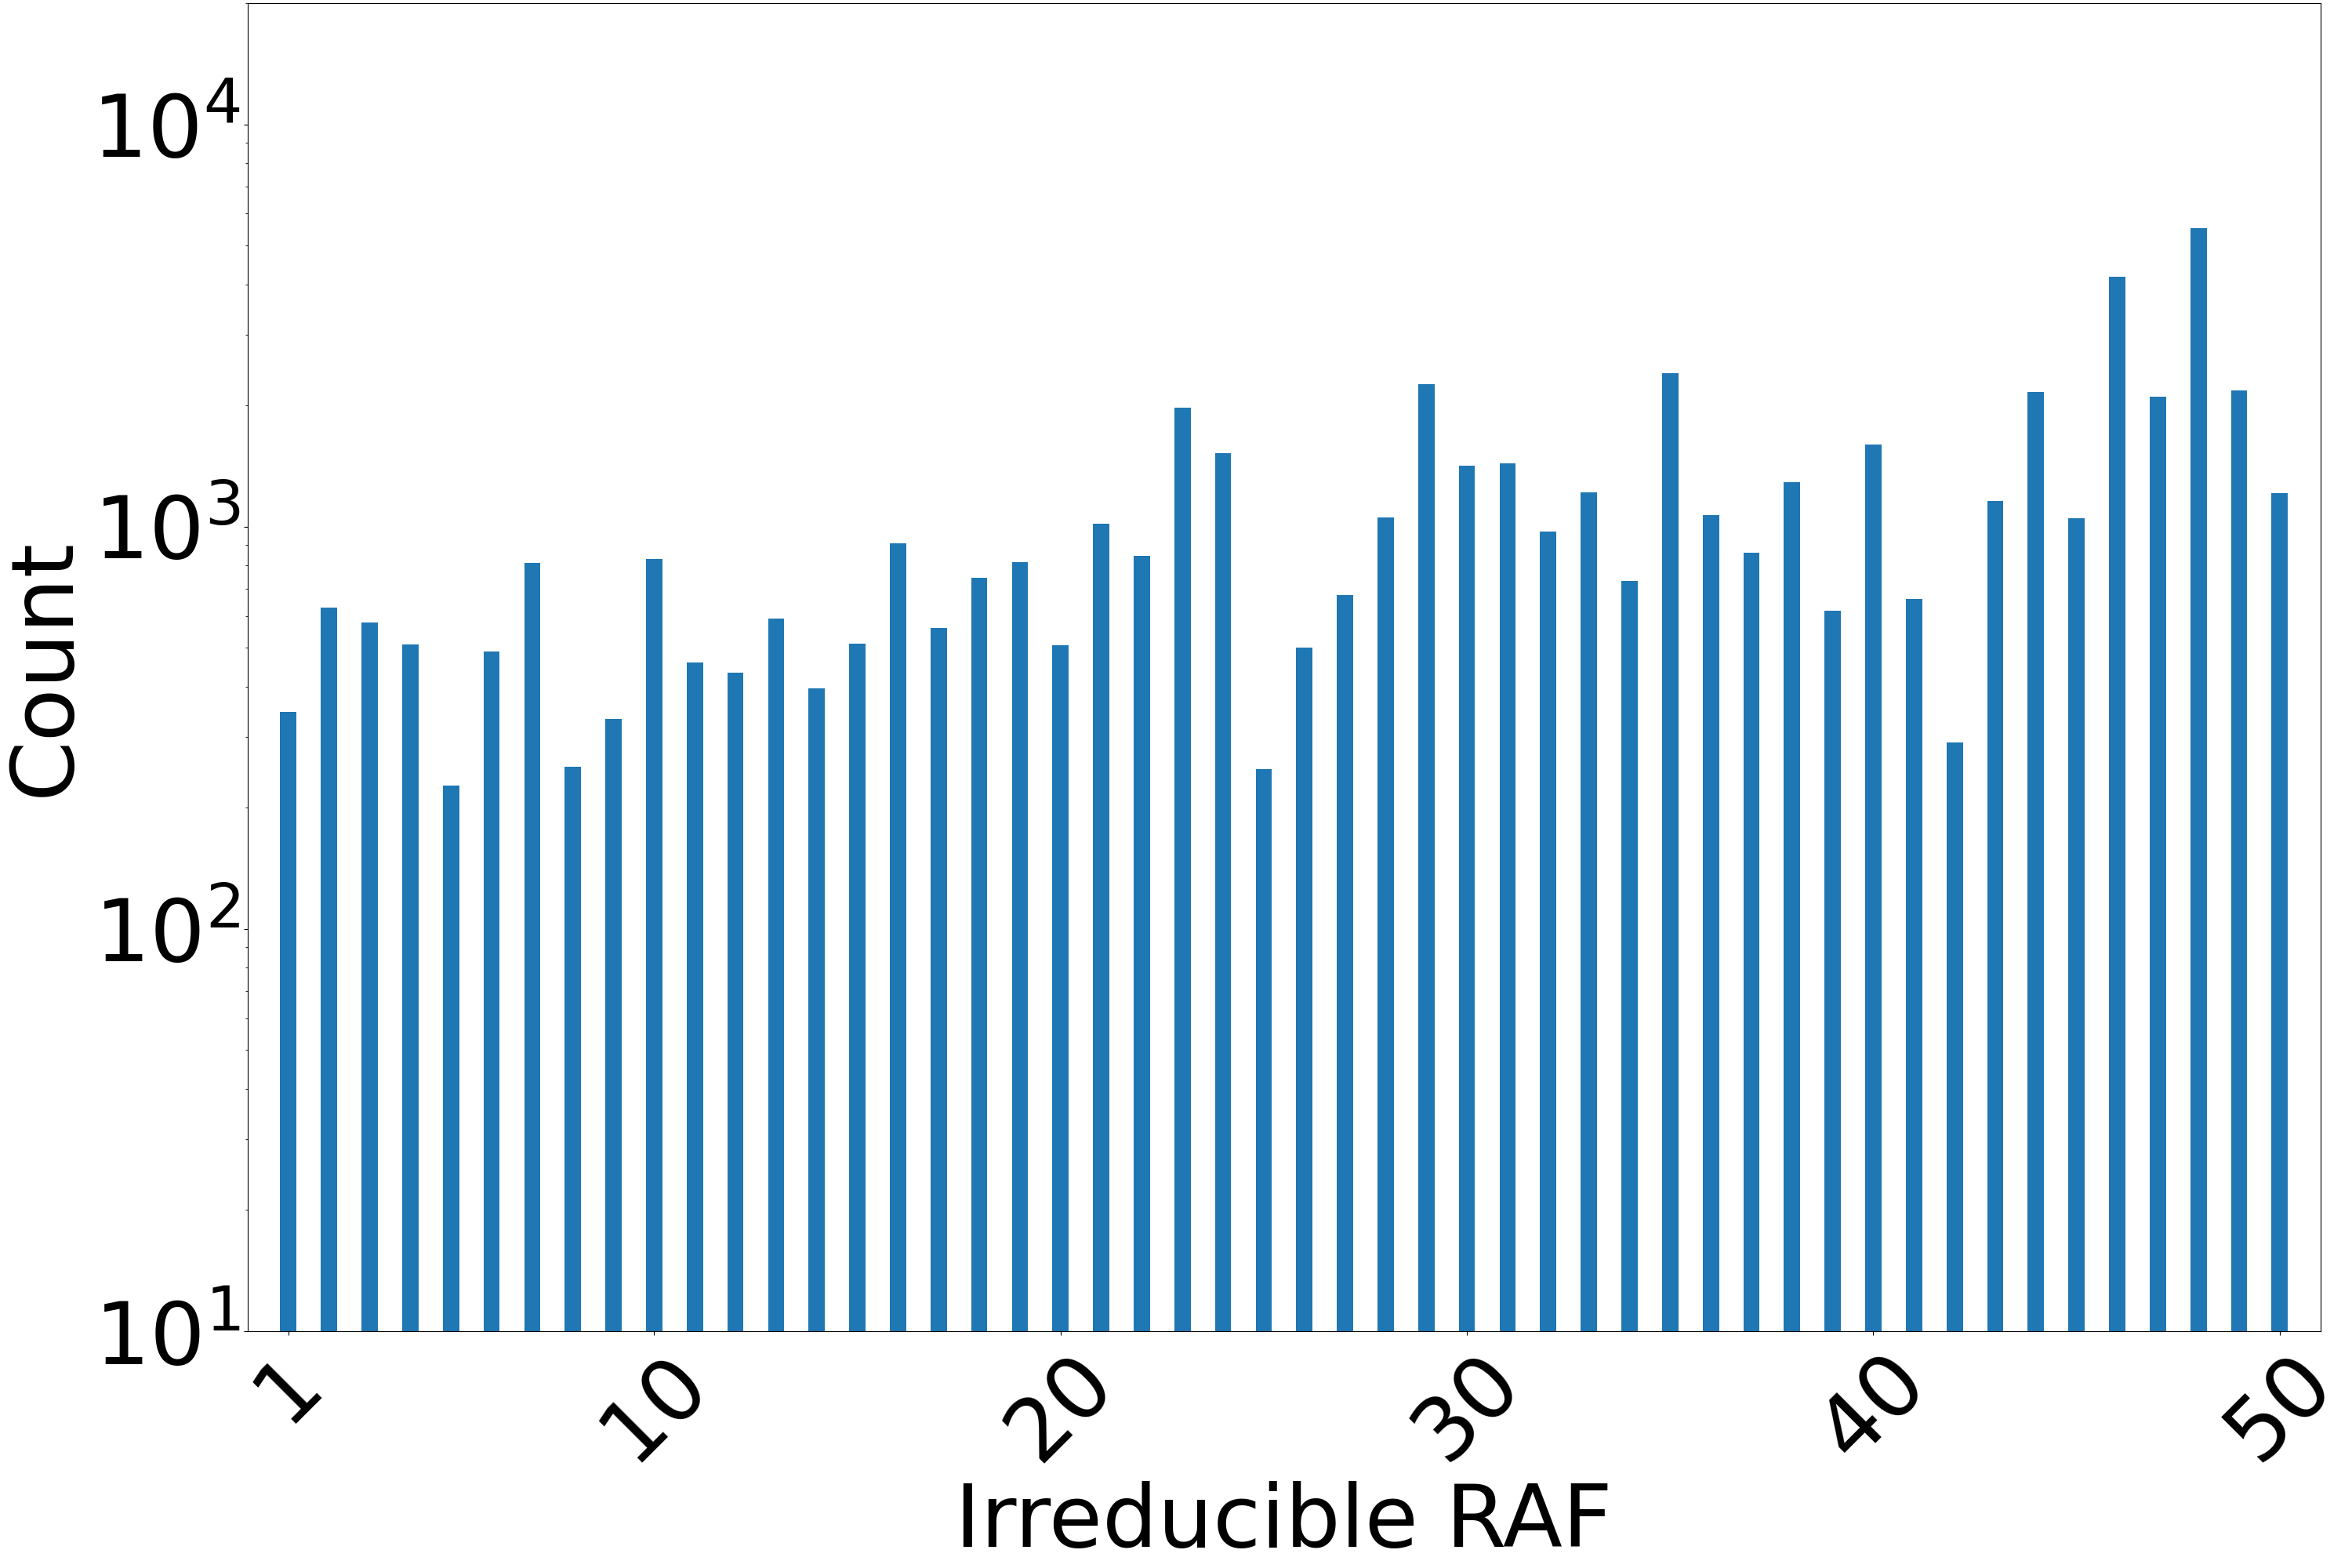
\includegraphics[width=0.9\textwidth]{./Pictures/n6iRAFCoresWFood.png}
    \end{minipage}%
    \hfill%
    \begin{minipage}[c]{0.5\textwidth}
      \centering
      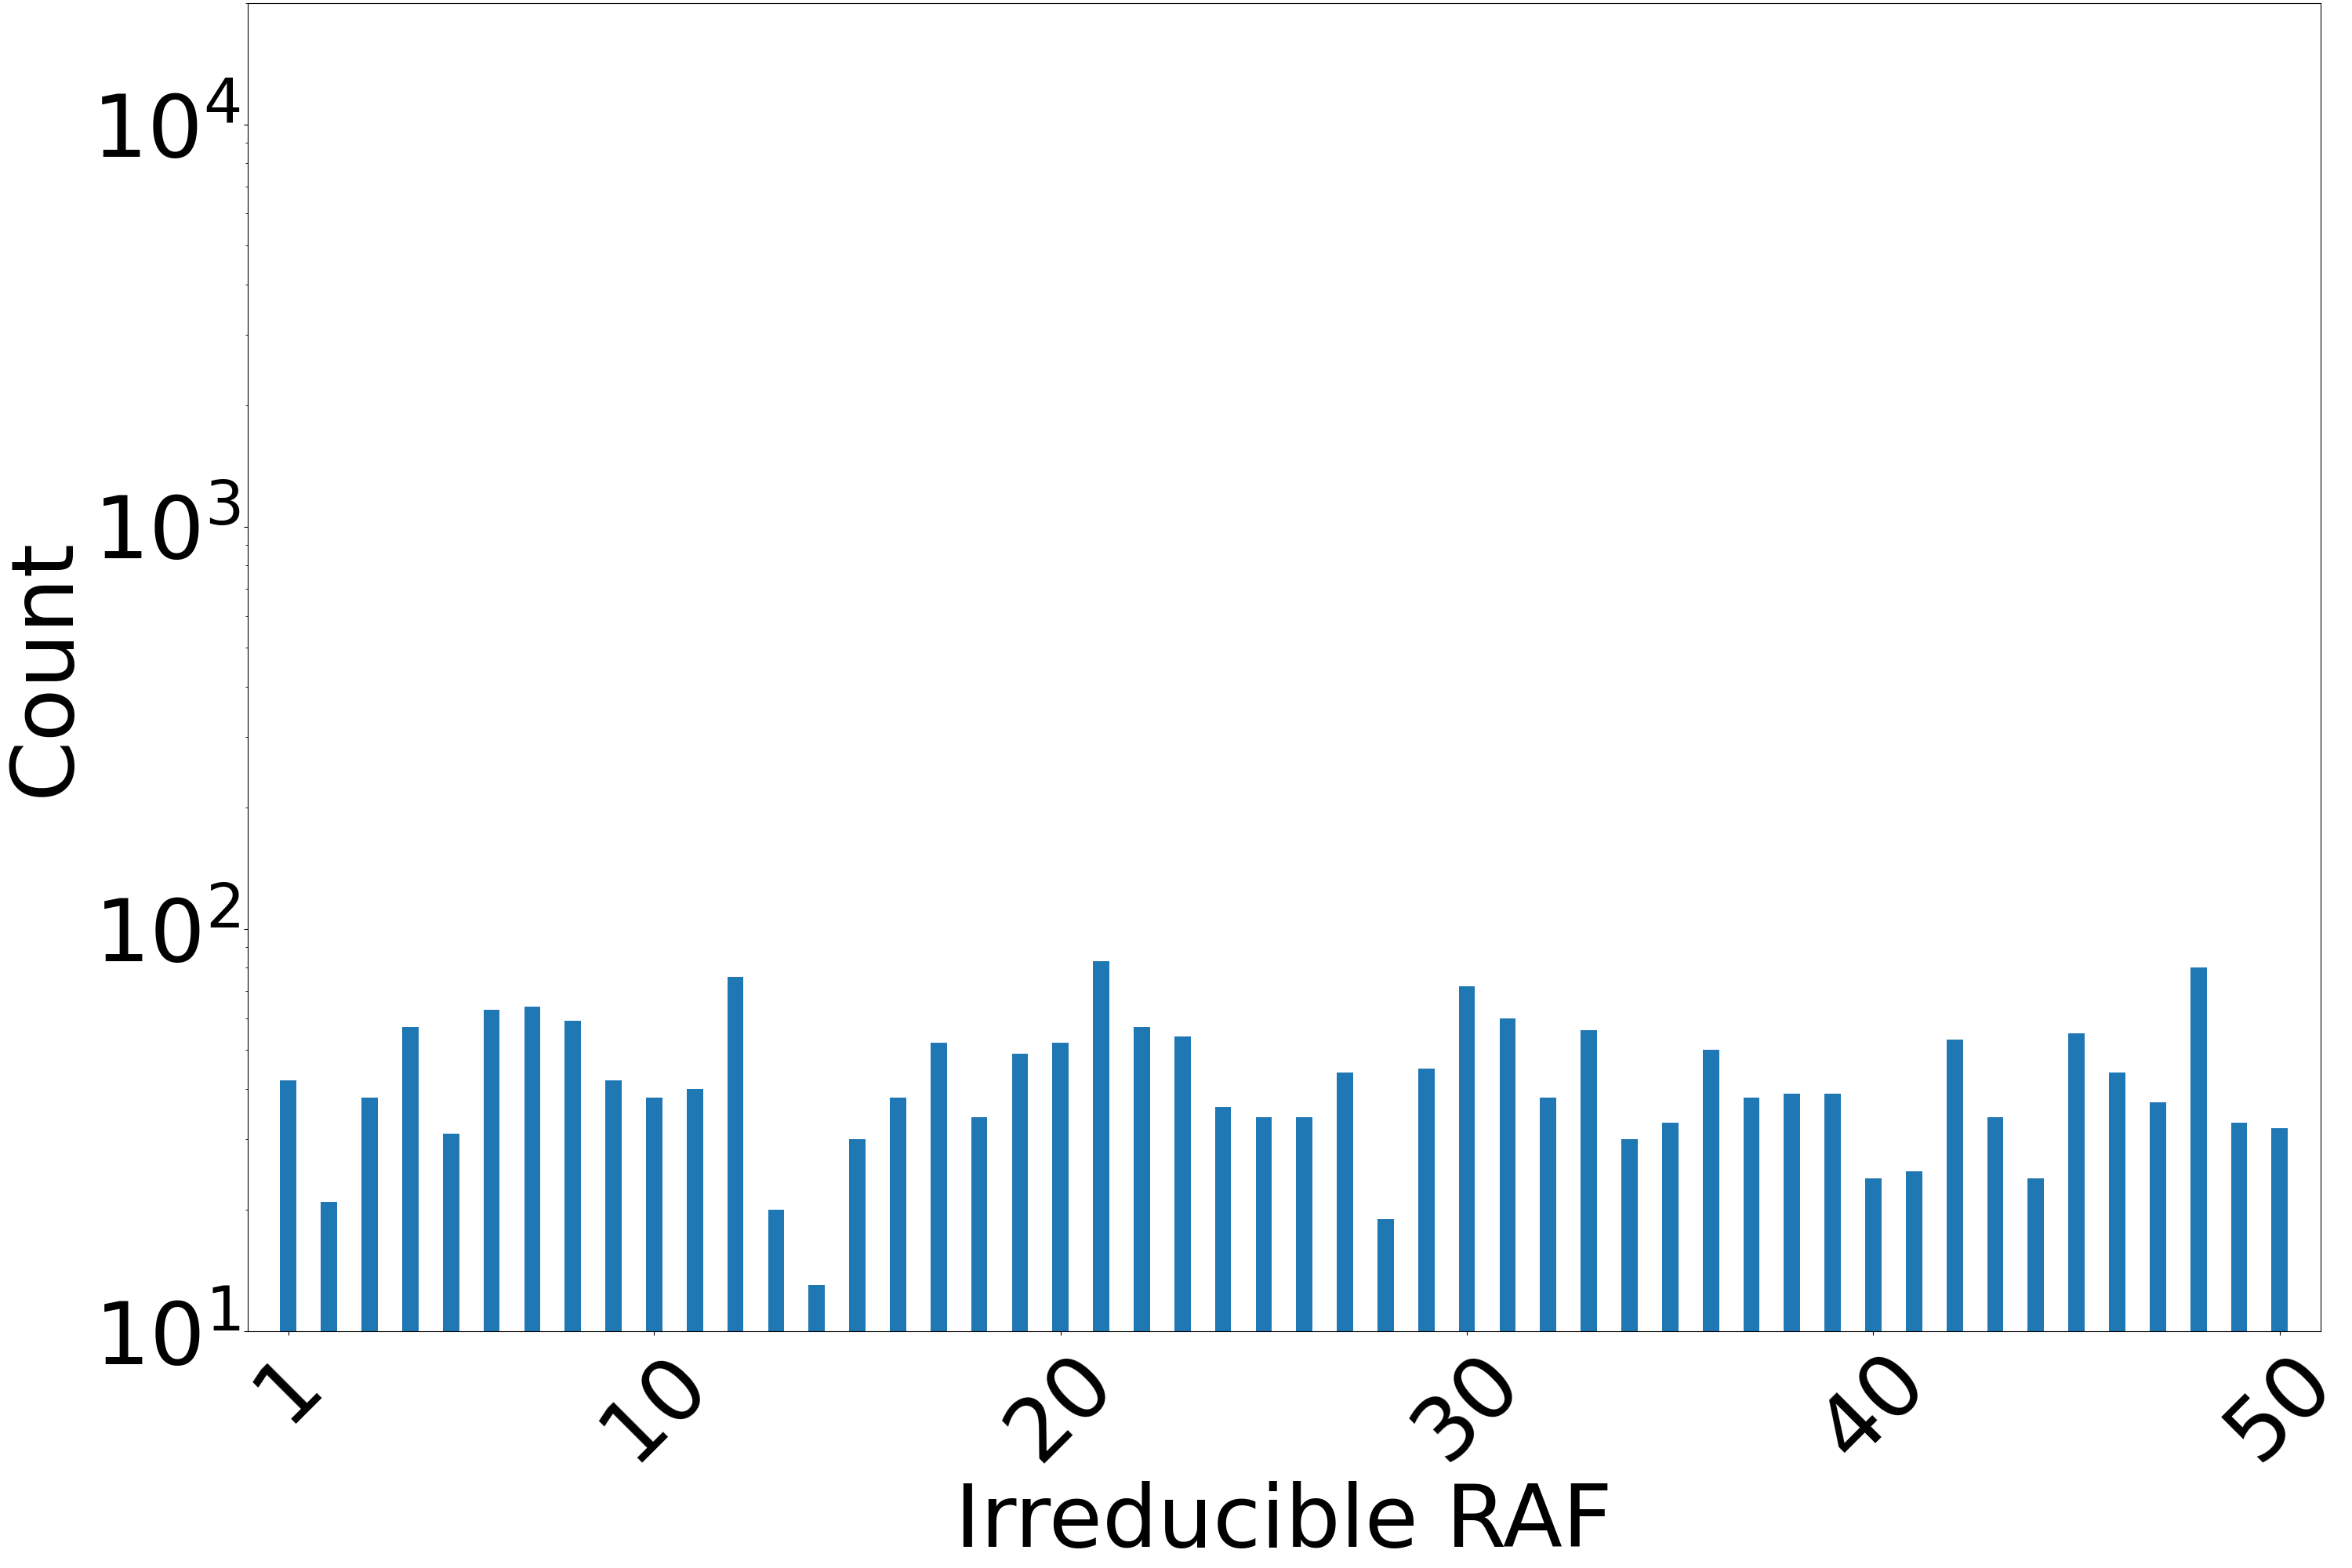
\includegraphics[width=0.9\textwidth]{./Pictures/n6iRAFirrevCoresWFoodRelevant.png}
    \end{minipage}
  \end{minipage}
%  \begin{minipage}[c]{\textwidth}
%    \centering
%    \begin{minipage}[c]{0.5\textwidth}
%      \centering
%      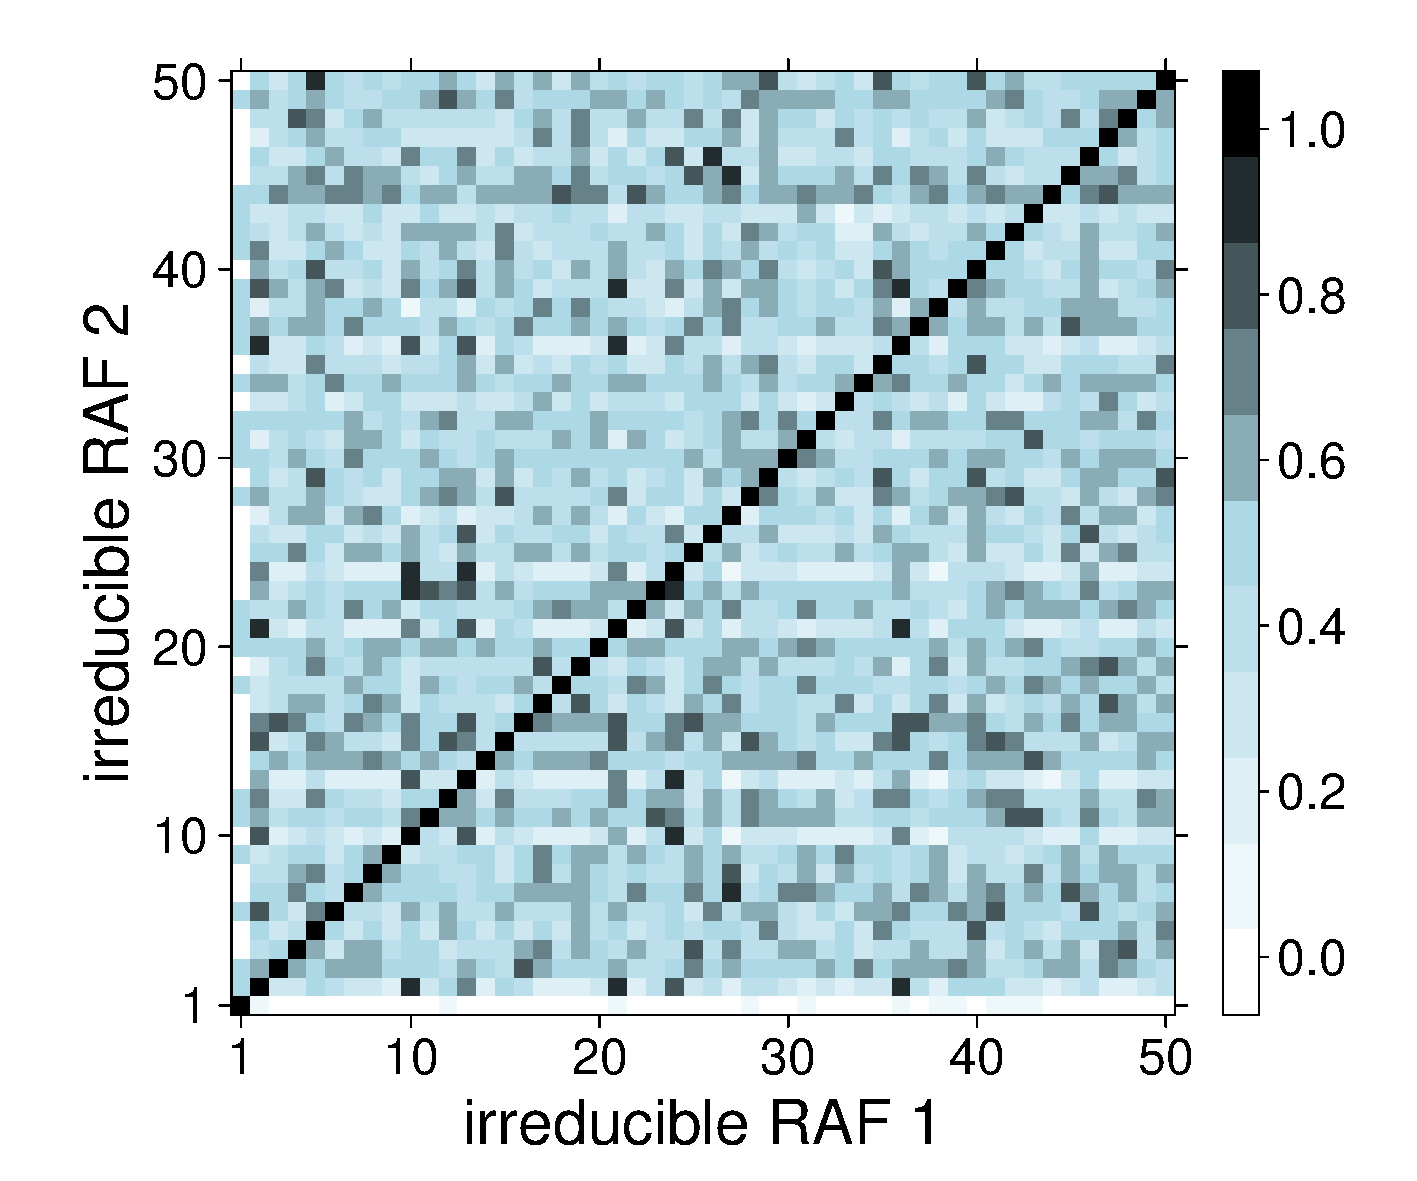
\includegraphics[width=\textwidth]{./Pictures/n5rev_overlap.pdf}
%    \end{minipage}%
%    \hfill%
%    \begin{minipage}[c]{0.5\textwidth}
%      \centering
%      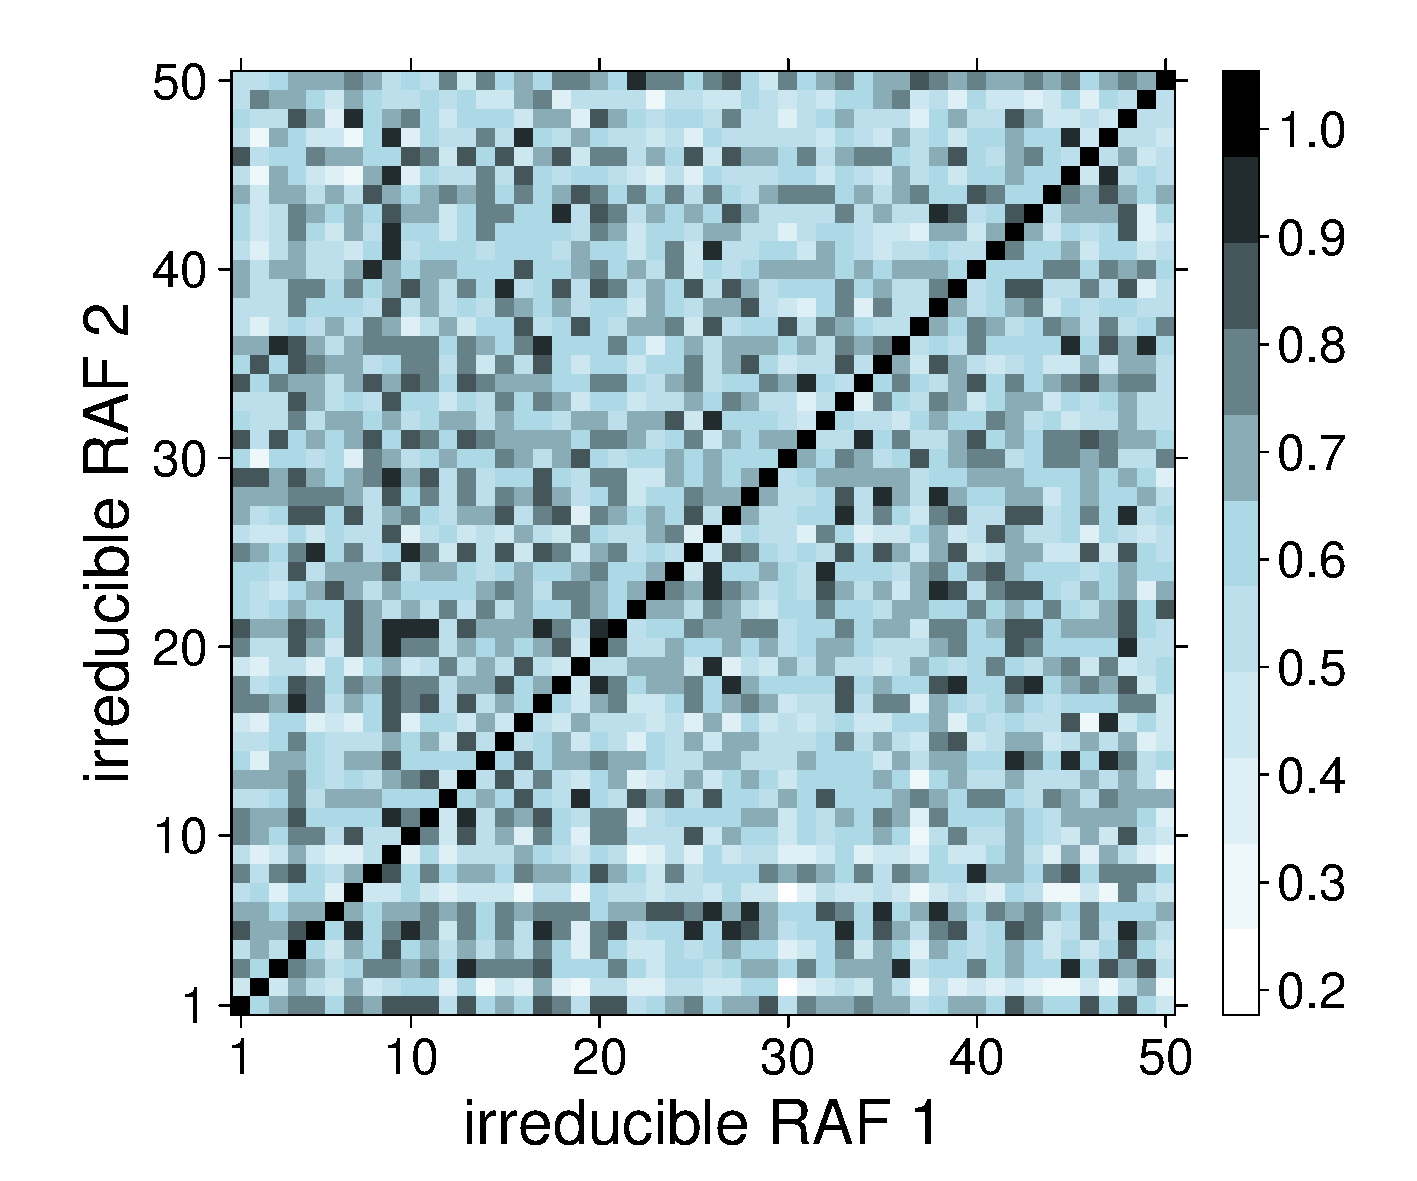
\includegraphics[width=\textwidth]{./Pictures/n5rev2_overlap.pdf}
%    \end{minipage}
%  \end{minipage}
  \begin{minipage}[c]{\textwidth}
    \centering
    \begin{minipage}[c]{0.5\textwidth}
      \centering
      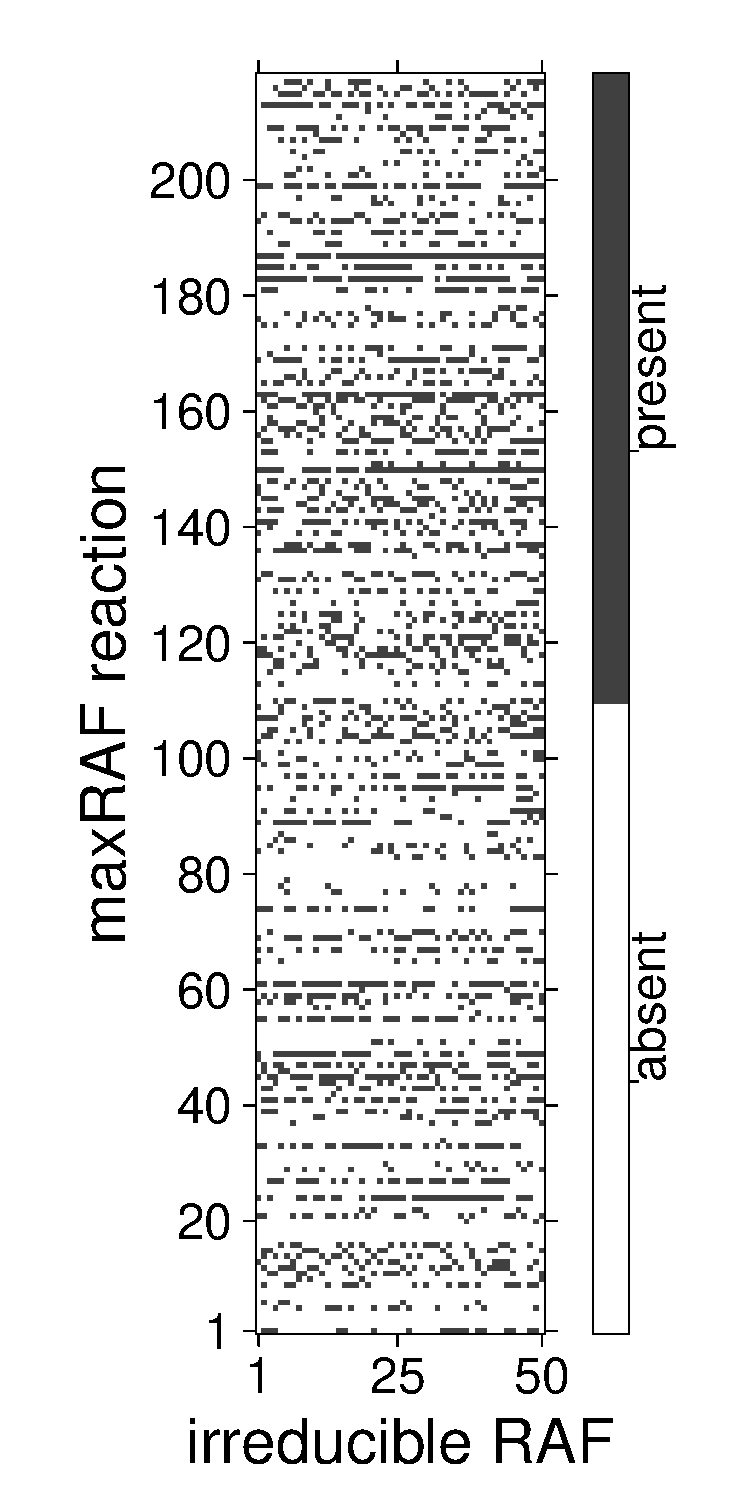
\includegraphics[width=0.8\textwidth]{./Pictures/n6_split_present.pdf}
    \end{minipage}%
    \hfill%
    \begin{minipage}[c]{0.5\textwidth}
      \centering
      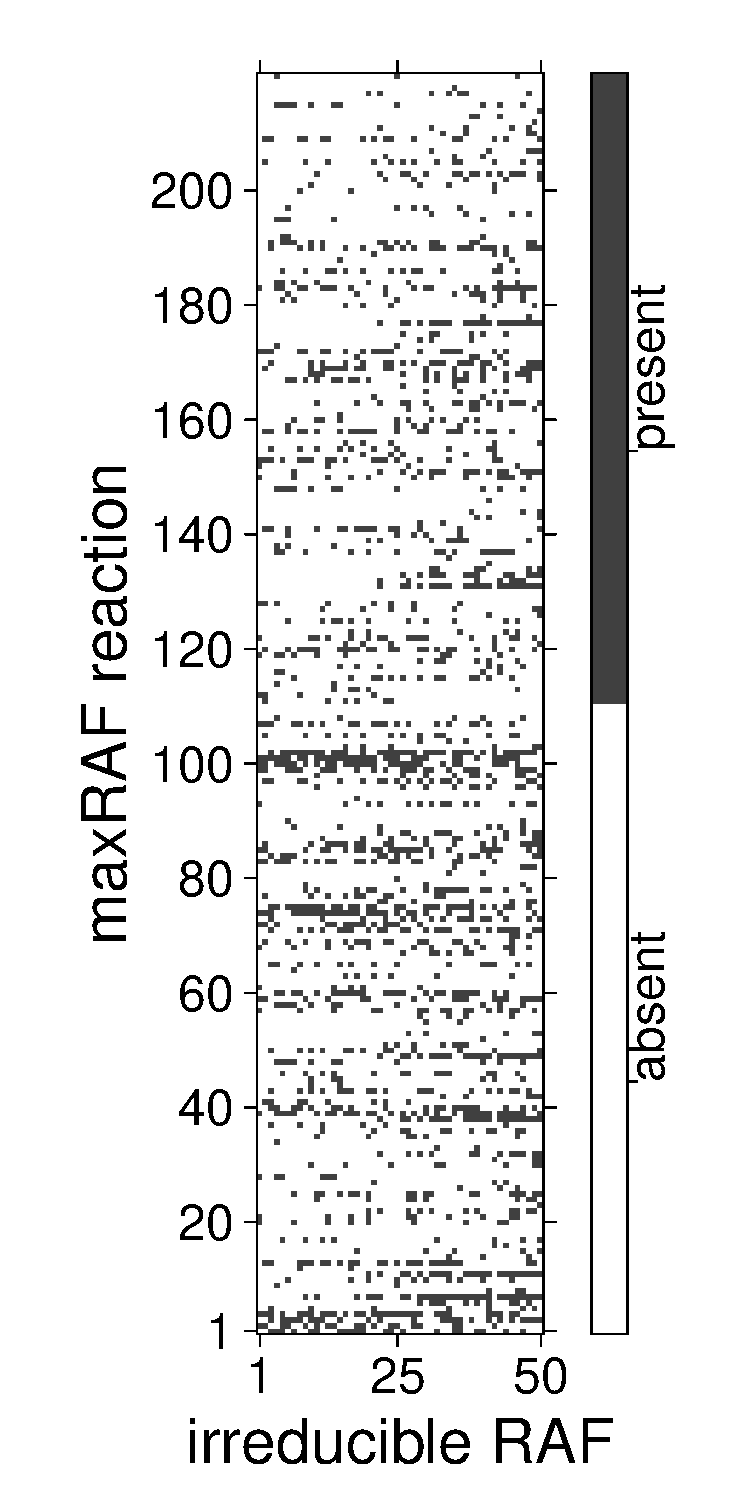
\includegraphics[width=0.8\textwidth]{./Pictures/n6_forw_present.pdf}
    \end{minipage}
  \end{minipage}	
  \caption{Irreducible RAFs typically contain many autocatalytic
      cores. \textbf{Top:} autocatalytic cores in individual irreducible RAFs. 
      % \textbf{Middle:} pairwise overlap of F-reactions between two irreducible RAFs.  
      \textbf{Bottom:} presence/absence of F-reactions from the maximal RAF in the
      individual irreducible RAFs.  The figure shows two instances of the
      binary polymer model with a fixed probability for any non-food species
      to catalyze any reaction of $p=0.01$ (\textbf{right}) and $p=0.008$
      (\textbf{left}) and maximum polymer length $6$ with \textbf{left} including 
      both ligation cleavage reactions, while \textbf{right} only ligation reactions. 
      See Sect.~\ref{sect:term} for the definition of terminology 
      and SI Sect.~\ref{S-sec:BinPol} for simulation details.}
  \label{fig:irrRAFCores}
\end{figure}


We first clarify in Sec.~\ref{sec:CRNCRS} the formal relationship between
the two underlying frameworks, chemical reaction networks (CRNs) and
catalytic reaction systems (CRSs), so that we may move freely between them:
Intuitively, CRSs can be viewed as quotient structures of associated
CRNs. We then study the structure of irreducible RAFs, particularly from a
graph-theoretic perspective, in Sec.~\ref{sec:RAF}. Through the quotient
relation between CRN and CRS, to each irreducible RAF we will associate an
exponentially large family of certain bipartite König
graphs. Sec.~\ref{sec:AutoCatIrrRAF} introduces stoichiometric
autocatalysis and our main result, Thm.~\ref{Thm:StrBlockCore}, which
states that every maximal \emph{strong block} \cite{grotschel_minimal_1979}
of each such bipartite graph contains an autocatalytic core. This
exponential correspondence provides an intuition for the large number of
autocatalytic cores observed in the irreducible RAFs of
Fig.\ref{fig:irrRAFCores}. We comment extensively on this aspect in
Sec.~\ref{sec:examples}. Nevertheless, we also show that this relationship
depends strongly on the type of network: we present an artificial
construction, which can produce examples containing any arbitrary number of
irreducible RAFs, yet invariably only one single autocatalytic core. We
conclude with a discussion of future directions.
 
\FloatBarrier

\section{Two Representations of Chemical Systems}\label{sec:CRNCRS}

Research on systems of chemical interactions has attracted considerable
attention, although formalizations lack consistency throughout the various
frameworks \cite{lohn_evolving_1998, steel_emergence_2000,
  feinberg_foundations_2019}. In particular, different authors have
introduced different notions of reactions \cite{muller_what_2022}. We
briefly overview here two approaches: \emph{Chemical Reaction Networks} and
\emph{Catalytic Reaction Systems}.

\subsection{Chemical Reaction Networks (CRNs)}
\label{sect:term}
A \emph{chemical reaction network} (CRN) $\Gamma \coloneqq (X,\CR)$ is a
tuple of two finite sets, a set of species $X$ and a set of reactions
$\CR$.  Any $r \in \CR$ is represented as an ordered association between a
nonnegative combination of reactant species to a nonnegative combination of
product species,
\begin{equation}\label{eq:reaction}
  \sum_{x\in X}\ s^-_{xr} \cdot x \quad
  \underset{r}{\longrightarrow} \quad
  \sum_{x\in X} \ s^+_{xr}\cdot x\,,
\end{equation}
where $s^{\pm}_{xr}$ are the reactant and product stoichiometry of the
molecule $x$ in the reaction $r$. The $|X|\times|\CR|$ \emph{stoichiometric
  matrix} $\SM$ encodes all \emph{net-stoichiometries}:
\begin{equation} 
  \SM_{xr} \coloneqq s^+_{xr}-s^-_{xr}.
\end{equation}

A \emph{sub-CRN} $\Gamma'\subseteq \Gamma$ is a tuple $\Gamma'=(X',\CR')$
with $X'\subseteq X$ and $\CR'\subseteq \CR$, where $r\in \CR'$ omits the
reference to species $x\not\in X'$, and the associated stoichiometric
matrix is denoted as $S[X',\mathcal{R}']$.

Clearly, stoichiometry and net-stoichiometry might not coincide, i.e.,
$s^{\pm}_{xr}\neq \pm S^{\pm}_{xr}$ for example due to
catalysis. From a chemical perspective, a \emph{catalyst} for $r$ is a
species $x\in X$ that appears on both sides of the stoichiometric equation
\eqref{eq:reaction}, i.e. with $s^-_{xr}s^+_{xr}\neq 0$, and that
additionally ``increases the rate of a reaction without modifying the
overall standard Gibbs energy change in the reaction''
\cite{gold_iupac_2025}.

However, a \emph{solvent} $x$ in a reaction $r$ may also formally satisfy
$s^-_{xr}s^+_{xr}\neq 0$ without being considered a catalyst
\cite{marx_nature_1999}, e.g. water in Br{\o}nstedt/Lowry's acid-base
theory \cite{eigen_proton_1964}. To be specific on the catalytic role a
species plays, we partition stoichiometries as in
\cite{golnik_bridging_2026} as
\begin{equation}
  s^{\pm}_{xr}=\sigma^{\pm}_{xr} + k_{xr}.
\end{equation}
It is readily verified that
$\SM_{xr} = s^+_{xr}-s^-_{xr} = \sigma^+_{xr} - \sigma^-_{xr}$, thus the
stoichiometric matrix is identically encoded in the coefficients
$\sigma^{\pm}_{xr}$.  Eq.~\ref{eq:reaction} can then be rewritten as:
\begin{equation}\label{eq:Mod.SmEq}
  \sum_{x\in X}\ \sigma^-_{xr} \cdot x + \left(\sum_{x\in X}\ k_{xr}
    \cdot x\right) \quad
  \underset{r}{\rightarrow} \quad
  \sum_{x\in X} \ \sigma^+_{xr} \cdot x +
  \left(\sum_{x\in X}\ k_{xr} \cdot x\right),
\end{equation}
We refer to species appearing in Eq.~\ref{eq:Mod.SmEq} with
$\sigma^{-}_{xr}>0$, $\sigma^{+}_{xr}>0$, and $k_{xr}>0$ as F-reactants,
F-products, and F-catalysts, respectively. The nomenclature ``F-catalysts''
is to distinguish this notion from the more loose definition of a catalyst
as a species that is both reactant and product, which is often also found
in CRN literature. We collect F-reactants, F-products, and F-catalysts in
the following sets:
\begin{equation}\label{eq:setsdef}
  \begin{split}
    \feducts(r) & \coloneqq \{x\in X \ | \ \sigma^-_{xr} > 0\}; \\
    \fproducts(r) & \coloneqq \{x\in X \ | \ \sigma^+_{xr} > 0\}; \\
    \cat(r)&\coloneqq \{(x, k_{xr})\ | \ x\in X,\; k_{xr}>0\}.
  \end{split}
\end{equation} 
For technical reasons (to be clarified below in Sec.~\ref{sec:CRS}), note
that the set of F-catalysts is defined as a set of pairs $(x,k_{xr})$ to
encode also the respective coefficient. For simplicity, with an abuse of
notation, we will write $x\in \cat(r)$ to refer to species $x$ for which
there exists a pair $(x,k_{xr})\in \cat(r)$. In a CRN, distinct reactions
$r_1\neq r_2$ may differ only in the F-catalysts
$\kappa_F(r_1)\neq \kappa_F(r_2)$ and share identical F-reactants and
F-products. For example, the hydrogenation of ethene to ethane can be
mediated by platinum, palladium, or nickel separately
\cite{crampton_ethylene_2016}. An example for co-catalysis, i.e., where the
orchestrated cooperation of two catalysts is required, is the dual-catalyst
system of palladium and copper in the Hoechst-Wacker process, where ethene
is oxidized to acetaldehyde \cite{jira_acetaldehyde_2009}. The idea that
one `same' chemical process, intended as a net-molecule transformation, can
be catalyzed by different catalysts has led to the different, although much
related, concept of Catalytic Reaction Systems, which we overview in the
text section.

\subsection{Catalytic Reaction Systems (CRS)}\label{sec:CRS}

\emph{Catalytic Reaction Systems} (CRS) \textit{sensu} 
Lohn \cite{lohn_evolving_1998} are defined as a triple 
\begin{equation}\mathbf{\Phi}\coloneqq (X, \FR, \cat(\FR)),
\end{equation}
where $X$ is again a set of species, and each $\fr\in\FR$ is defined as a
net-molecule transformation
\begin{equation}\label{eq:FReacEq}
  \sum_{x\in X}\ \sigma^-_{x\fr} \cdot x \quad
  \underset{\fr}\longrightarrow \quad
  \sum_{x\in X}\ \sigma^-_{x\fr} \cdot x,
\end{equation}
where $\sigma^\pm_{x\fr}\ge 0$ are again nonnegative stoichiometric
coefficients. The sets of F-reactants $\feducts(\fr)$ and F-products
$\fproducts(\fr)$ of an F-reaction $\fr$ are defined identically as in
\eqref{eq:setsdef} for CRNs.  The main difference with the CRN setting are
the \emph{catalyzations} $\cat(\FR)=\{ \cat(\fr) \}_{\fr\in\FR}$.  For a
single F-reaction $\fr$, the set of catalyzations $\cat(\fr)$ is defined as
$\cat(\fr)=\{c_\fr\}$, where each catalyzation $c_\fr$ is in turn a set of
pairs $(x,k^{c}_{x\mathbf{r}})$:
\begin{equation}\label{eq:CatCFR}
    c_\fr\coloneqq \{(x_1,k^c_{x_1\mathbf{r}}),\ldots, (x_n,k^c_{x_n\fr})\}.
\end{equation}
where $k^{c}_{x\fr}>0$ is a positive coefficient. Again, for simplicity and
with abuse of notation, we will write $x\in c_\fr$ for a species $x$ such
that there exists $k^c_{x\fr}$ for which $(x,k^c_{x\fr})\in c_{\fr}$.  We
call an $\fr\in \FR$ \emph{F-reaction} to distinguish it from the CRN
reactions \eqref{eq:Mod.SmEq}. A CRS
$\mathbf{\Phi}'\coloneqq (X', \FR', \cat'(\FR'))$ is a \emph{sub-CRS} of
$\mathbf{\Phi}\coloneqq (X, \FR, \cat(\FR))$ if $X\subseteq X'$,
$\FR'\subseteq\FR$, $\cat'(\FR')\subseteq \cat(\FR)$.

Finally, a comparison between a CRN reaction \eqref{eq:Mod.SmEq} with a CRS
F-reaction \eqref{eq:FReacEq} and the definition of catalyzations set
$\cat$ suggests the following formalization of the relation between a CRN
and a CRS.

\paragraph{From a CRN $\Gamma=(X,\mathcal{R})$ to a CRS
  $\mathbf{\Phi}\coloneqq (X, \FR, \cat(\FR))$.}
Consider the equivalence relation $\sim$ on CRN reactions defined as
\begin{equation}\label{eq:EqRel}
    r_1 \sim r_2 \quad \text{if $\sigma_{xr_1}^{\pm}=\sigma_{xr_2}^{\pm}$ for any $x\in X$.}
\end{equation}
To each CRN $\Gamma=(X,\mathcal{R})$ we associate a CRS
$\mathbf{\Phi}(\Gamma)\coloneqq (X, \FR, \cat(\FR))$ where $\FR$ is just
the quotient set of $\mathcal{R}$ over the equivalence relation $\sim$,
i.e.
\begin{equation}
    \FR=\dfrac{\mathcal{R}}{\sim}.
\end{equation}
In particular, an F-reaction in a CRS is just an equivalence class of CRN
reactions, $\fr=[r]_{\sim}$. Each catalyzation $c$ is then just the set of
F-catalysts $c(\mathbf{r})=\cup_ {r\in \fr}\{\cat(r)\}$.

\paragraph{From a CRS $\mathbf{\Phi}\coloneqq (X, \FR, \cat(\FR))$ to a CRN
  $\Gamma=(X,\mathcal{R})$.} Viceversa, by rolling back the previous
argument, to each CRS $\mathbf{\Phi}\coloneqq (X, \FR, \cat(\FR))$ we
associate a CRN $\Gamma (\mathbf{\Phi})=(X,\mathcal{R})$, where each
reaction $r\in \mathcal{R}$ corresponds to a pair $(\fr,c_\fr)$, naturally
defined from \eqref{eq:FReacEq}, setting $\cat(r)=c_\fr$, and defining $r$
via \eqref{eq:Mod.SmEq} with $\sigma^{\pm}_{xr}=\sigma^{\pm}_{x\fr}$.

By construction, it is clear that 
\begin{equation}
  \Gamma(\mathbf{\Phi}(\Gamma))=\Gamma \quad \text{and}
  \quad \mathbf{\Phi}(\Gamma(\mathbf{\Phi))}=\mathbf{\Phi}.
\end{equation}
Moreover, since $\FR$ is a quotient set from $\mathcal{R}$, we have that
$|\FR| \le |\mathcal{R}|$, with equality achieved if, and only if, each
F-reaction $\fr$, viewed as an equivalence on $\mathcal{R}$, consists only
of one element, i.e.  $\fr=[r]_{\sim}=\{r\}$.

\section{Reflexively Autocatalytic Food-Generated Sets}\label{sec:RAF}

Catalytic Reaction Systems $(X,\FR,\cat(\FR))$ are the framework on which
the notion of \emph{Reflexively Autocatalytic F-generated Sets} (RAFs) has
been introduced \cite{steel_emergence_2000, hordijk_detecting_2004}. Their
definition relies on the concept of \emph{closure}. The closure
$\closure{\RAF}{X'}$ of a species set $X' \subseteq X$ w.r.t.\ to a
F-reaction set $\RAF \subseteq \FR$ is the unique inclusion-minimal subset
$Y\subseteq X$ containing $X'$ such that for any
$\fr\in \RAF: \feducts(\mathbf{r})\subseteq Y \Rightarrow
\fproducts(\mathbf{r})\subseteq Y$. In symbols:
\begin{equation}\label{eq:Closure}
  \closure{\RAF}{X'} \coloneqq \min_{\subseteq} \{Y  \ | \ X'\subseteq Y \subseteq X,\;
  \feducts(\mathbf{r}) \subseteq Y \Rightarrow \fproducts(\mathbf{r}) \subseteq Y \ \forall
  \mathbf{r}\in \RAF\}.
%%  %}_{\eqqcolon \mathfrak{C}_{\RAF}(X')}
\end{equation}
A Reflexively Autocatalytic F-generated set (RAF) is then defined as
follows \cite{hordijk_required_2011}:

\vspace{6pt}
\begin{definition}[RAF]\label{def:RAF}
  Let $(X,\FR,\cat(\FR))$ be a CRS with a specified \emph{food set} $\food\subseteq X$. A 
  set $\RAF\subseteq \FR$ is called
  \vspace{6pt}
  \begin{itemize} 
  \item[i.]{\emph{Reflexively Autocatalytic} (RA) if, for each
      $\mathbf{r}\in \RAF$,
      there exists at least one catalyzation $c\in \cat(\mathbf{r})$ such that $c \subseteq \closure{\RAF}{\food}$;}\\[-1.0em]
  \item[ii.]{\emph{\food-generated} (F) if $\feducts(\RAF)\subseteq
      \closure{\RAF}{\food}$;}\\[-1.0em]
  \item[iii.]{\emph{Reflexively Autocatalytic and $\food$-generated}
    (RAF) if both i. and ii. hold.}
  \end{itemize}
\end{definition}
%\vspace{6pt}
\begin{remark}\label{rmk:RAFCRN}
  Def.~\ref{def:RAF} does not formally require the formalism of CRS, and it
  can be stated identically for CRN so that we may naturally
  speak of sets of food-generated CRN reactions, as well. This route was
  undertaken e.g. in \cite{golnik_bridging_2026}.
\end{remark}
We also remark that Property~$ii.$ together with the definition of the
closure, Eq.~\eqref{eq:Closure}, directly implies that all F-products of
any F-reaction $\fr\in \RAF$ are also contained in $\closure{\RAF}{\food}$,
thus $\fproducts(\fr)\subseteq \closure{\RAF}{\food}$. Finally, it is also
worthwhile noting that Property~$i.$ and ~$ii.$ are independent of each
other. In particular, Property~$ii.$ depends only on $\food$ and $\RAF$,
and not on the catalyzations. This reveals an inherent freedom in the
definition of catalyzations of a RAF, as the following Lemma underlines.

\vspace{6pt}
\begin{lemma}\label{lem:ArbCat}

  Let $X$ be a set of species and $\FR$ be a set of $F$-reactions on
  $X$. Then, for any $\food$-generated set $\RAF$ there exist infinitely
  many sets of catalyzations $\{\cat(\FR)_i\}$ which make $\RAF$ a RAF in
  the CRS $(X,\FR,\cat (\FR)_i))$, for any $i$.
\end{lemma}
\begin{proof}
  To define such valid set of catalyzations $\cat(\FR)$, it is sufficient
  to arbitrarily assign to each F-reaction $\mathbf{r}$ any set
  $\{c_j(\fr)\}$ of sets of species $c_j(\fr)\subseteq X$. For
  $\mathbf{r}\in \RAF$, we shall further require that at least one set
  $c_{j^*}(\fr)$ consists only of species that are in the closure,
  i.e. ${c_{j^*}}(\fr)\subseteq \closure{\RAF}{\food}$. Obviously, any such
  choice of catalyzations renders $\RAF$ Reflexively Autocatalytic. It is
  also obvious that such arbitrary assignments are infinite.
\end{proof}

\subsection{A preorder on RAFs}

The reactions of a RAF can be partially ordered such that for each
$x\in\feducts(\mathbf{r})$ we have $x\in\food$ or there is a reaction
$\mathbf{r}'\prec \mathbf{r}$ such that $x\in\fproducts(\mathbf{r}')$.  We
construct one such order that is reminiscent of a breadth-first search.  To
this end, we define sequences of nested species subsets $(X'_0, ..., X'_n)$
where $X'_0=\food$ and
\begin{equation}\label{eq:speciesSubSet}
  X'_i\coloneqq X'_{i-1}\cup \bigcup_{\feducts(\mathbf r)\subseteq X'_{i-1}}
  \fproducts(\mathbf r).
\end{equation} This iterative process builds 
$\closure{\RAF}{\food}$ in a finite number of steps as long as
$\vert \RAF\vert <\infty$. A formal account of this procedure is
given in the Supplemental Material.

These ordered sequences define a \emph{generation reaction-index}
$\gamma(\mathbf{r})$ where an F-reaction $\mathbf{r}$ happens for the first
time, i.e.
\begin{equation}\label{def:genreactionindex}
  \gamma(\mathbf{r})\coloneqq \operatorname{min} \{i \; | \; \feducts(\mathbf{r})\subseteq X'_i\} + 1,
\end{equation} 
where the index is shifted by one for normalization, so that the
\emph{first} generation corresponds to index $\gamma(\mathbf{r})=1$.
Similarly, the sequences define a \emph{generation species-index} $g(x)$
where a non-food species $x\not\in \food$ is produced for the first time,
i.e. \begin{equation} g(x)= \operatorname{min} \{i \; | \; x\in
  X'_i\}.\end{equation} Clearly, the total order $\le$ on the natural
numbers induces a preorder $\preccurlyeq$ on $X\setminus \food$ and a
preorder $\preceq$ on $\mathbf{R}$
\begin{equation}
\begin{cases}
  x_1\preccurlyeq x_2 \quad&\text{if}\quad \sgen(x_1) \leq \sgen(x_2);\\
  \fr_1\preceq \fr_2 \quad &\text{if} \quad \rgen(\fr_1) \leq \rgen(\fr_2).
\end{cases},
\end{equation}
which we refer to as \emph{generation orders} on species and F-reactions,
respectively. By Remark~\ref{rmk:RAFCRN}, we will use the index $\gamma$
indistinctly also for reactions \eqref{eq:Mod.SmEq} in a CRN setting. In
particular, from the definition of $\gamma$ it follows consistently that
$\gamma(r_1)=\gamma(r_2)$ whenever $r_1\sim r_2$ and thus
$\gamma(r_1)=\gamma(\fr)$ for $\fr=[r_1]_\sim$.

\TODO{[TBA comment on preorder vs partial order?]}

We conclude this section with the formal definition of CAFs sets.
\vspace{6pt}
\begin{definition}\label{def:CAF}
  A \emph{constructively autocatalytic and food-generated} set (CAF) is a
  RAF such that for each F-reaction $\fr$ all $x\in \feducts(\fr)$ satisfy
  $\sgen(x)<\rgen(\fr)$ and there is at least one catalyzation
  $c\in \cat(\mathbf{r})$ such that all F-catalysts $x\in c$ satisfy
  $\sgen(x)< \rgen(\fr)$.
\end{definition}

\subsection{Irreducible RAFs}\label{sec:IrrRAF}

For a CRS $(X,\FR,\cat(\FR))$ with food-set $\food\subseteq X$, 
the minimality of the RAF structure $\RAF$ with respect to its F-reactions, 
has been investigated in \cite{steel_minimal_2013}. To this aim, the 
notion of \emph{irreducible RAFs} has been introduced.

\vspace{3mm}
\begin{definition}[Irreducible RAF]\label{def:irrerRAF}
  Let $\RAF$ be a RAF of the CRS $(X,\FR,\cat(\FR))$. $\RAF$ is
  \emph{irreducible} if no subset $\RAF'\subset \RAF$ determines a RAF.
\end{definition}

\emph{Example.} Consider a species set $X=\{x_0,...,x_{n+1}\}$ with food 
set $\food=\{x_0\}$ and a sequence of $n+1$ F-reactions
\begin{equation}\label{eq:ExReacSeq}
x_i + (x_{i+1})\quad\underset{\fr_i}\longrightarrow\quad x_{i+1}+(x_{i+1}),
\end{equation}
such that the F-product $x_{i+1}$ is also the F-catalyst (indicated in
brackets).  Clearly, any set $\RAF_k$ of the form
$\RAF_k\coloneqq \{\fr_0,\ldots, \fr_k\}$, with $k\leq n$ satisfies
Def.~\ref{def:RAF} and it is thus a RAF. In particular, $\RAF_0=\{\fr_0\}$
is an irreducible RAF.


The minimality condition imposed on the set of F-reactions via
Def.~\ref{def:irrerRAF} directly yields the following two structural lemmas.
\vspace{6pt}
\begin{lemma}\label{lem:OneFReacPerRAF}
  Let $(X,\FR,\cat(\FR))$ be a CRS with food-set $\food\subseteq X$. An
  irreducible RAF $\RAF$ never contains two distinct F-reactions $\fr_1$
  and $\fr_2$ such that either of the following conditions hold:
  \begin{enumerate}
  \item their F-reactants and F-products coincide: 
  \begin{equation}\label{eq:netreaction}
    \feducts(\fr_1)=\feducts(\fr_2) \qquad\text{and}\qquad
    \fproducts(\fr_1)=\fproducts(\fr_2) 
  \end{equation}
\item the F-reactants of $\fr_1$ coincides with the F-products of $\fr_2$,
  and vice versa:
  \begin{equation}\label{eq:inverse}
    \feducts(\fr_1)=\fproducts(\fr_2) \qquad\text{and}\qquad
    \feducts(\fr_2)=\fproducts(\fr_1) 
  \end{equation}
\end{enumerate}
\end{lemma}
\begin{proof}
  Indirectly assume there exist two F-reactions $\fr_1,\fr_2\in \RAF$ such
  that either \eqref{eq:netreaction} or \eqref{eq:inverse} holds and
  assume, without loss of generality, that $\fr_1\preceq \fr_2$. Consider
  the set $\RAF'\coloneqq \RAF \setminus \fr_2$. Since
  \eqref{eq:netreaction} (resp. \eqref{eq:inverse} holds, it follows that
  $\closure{\RAF}{\food} = \closure{\RAF'}{\food}$, since $\fr_1$ and
  $\fr_2$ have the same F-reactants and F-products (resp. since the
  F-products of $\fr_2$ are F-reactants of $\fr_1$). Therefore, $\RAF'$ is
  (i) Reflexively Autocatalytic, since $\RAF$ is, and (ii) is
  $\food$-generated; in particular, $\RAF'$ is a RAF which contradicts
  $\RAF$ being irreducible.
\end{proof}
We remark that \eqref{eq:inverse} in particular formally excludes the presence in any irreducible RAF of two F-reactions that are each other's reverse. Writing a pair of reverse F-reactions as defined by \eqref{eq:inverse} as
\begin{equation}\label{eq:reversereac}
  \fr_1 = \bar{\fr}_2  \qquad\text{and}\qquad \fr_2 = \bar{\fr}_1
\end{equation}
and a set of reverse F-reactions as
\begin{equation}\label{eq:reverseset}
  S = \{\fr_1,\fr_2,\ldots,\fr_k\} \Rightarrow \bar{S} = \{\bar{\fr}_1,\bar{\fr}_2,\ldots,\bar{\fr}_k\}
\end{equation}
we can also state the following result.
\vspace{6pt}
\begin{lemma}\label{lem:noReverseIrrRAF}
  Let $(X,\FR,\cat(\FR))$ be a CRS with food-set $\food\subseteq X$, and $\RAF \subset \FR$ a (non-trivial) irreducible RAF. For any subset $S \subseteq \RAF$, the set $\RAF' = (\RAF \setminus S) \cup \bar{S}$ is not an irreducible RAF.
\end{lemma}
\begin{proof}
  First assume that $\RAF$ with one (arbitrary) F-reaction $\fr_i$ reversed is an irreducible RAF $\RAF'$. That means that $\feducts(\bar{\fr}_i) = \fproducts(\fr_i) \subset \closure{\RAF}{\food}$. However, that means that $\RAF \setminus \{\fr_i\}$ is also a RAF, contradicting the fact that $\RAF$ is irreducible.
  Alternatively, it could be that $\feducts(\bar{\fr}_i) \not\subset \closure{\RAF}{\food}$, but that by reversing some other F-reaction $\fr_j \in \RAF$ it will be. But then the first argument can be applied to $\fr_j$, or otherwise it leads to an increasing sequence of reversed F-reactions where (i) some reversed F-reaction $\bar{\fr}_k$ requires an F-reactant that is an F-product of an earlier reversed F-reaction, or (2) for some reversed F-reaction $\bar{\fr}_k$ it is the case that $\feducts(\bar{\fr}_k) \subset \food$. In case (i) $\RAF'$ cannot be an irreducible RAF as it is not $\food$-generated (having a cycle of F-reactions where each F-reaction has an F-reactant that is only produced by the previous F-reaction in the cycle), and in case (ii) it follows that $\fproducts(\fr_k) \subset \food$, which contradicts the fact that $\RAF$ is irreducible.
\end{proof}
In words, given an irreducible RAF $\RAF$, there is no subset of F-reactions $S \subseteq \RAF$ such that when all F-reactions in the subset $S$ are reversed, the resulting set is also an irreducible RAF. The only exception is an irreducible RAF consiting of a single reaction where all F-reactants, F-products, and at least one catalyst are all in the food set $\food$.

Since a RAF is defined in Def.~\ref{def:RAF} as a subset of F-reactions,
Def.~\ref{def:irrerRAF} imposes a minimality condition only on the set of
F-reactions. However, motivated by the fact that in the CRN-setting
different catalyzationsof the same F-reaction correspond to different
reactions, we also consider irreducible RAFs $\RAF$ with a minimal number
of catalyzations while conserving irreducibility.

For any $\food$-generated set $\RAF$, Lemma~\ref{lem:ArbCat} shows indeed
that infinitely many catalyzations exist that render $\RAF$ a
RAF. Complementarily, we address which catalyzation subsets
$\cat'(\FR)\subset \cat(\FR)$ preserve the fact that an $\food$-generated
set $\RAF$, which is an irreducible RAF in the CRS $(X,\FR, \cat(\FR))$, is
still an irreducible RAF in the CRS $(X,\FR, \cat'(\FR))$.  The following
Lemma shows that $\cat'(\FR)$ can always be chosen such that
$|\cat'(\fr)|=1$ for all F-reactions $\fr\in \RAF$.

\vspace{6pt}
\begin{lemma}\label{lem:mono}
  Let $\mathbf{\Phi}\coloneqq (X,\FR,\cat(\FR))$ be a CRS with specified
  \emph{food set} $\food\subseteq X$ and let $\RAF$ be an irreducible
  RAF. Then $\RAF$ is also an irreducible RAF in any CRS
  $(X, \FR,\cat'(\FR))$ where the catalyzations
  $\cat'(\FR)\subseteq\cat(\FR)$ satisfy:
  \begin{equation}\label{eq:casesmono}\cat'(\fr)=\begin{cases}
    \{c\}\text{ with $c\subseteq \closure{\RAF}{\food}$}\quad
    &\text{if $\fr\in \RAF$,}\\ 
    \cat(\fr)&\text{otherwise.}
  \end{cases}, 
\end{equation}
\end{lemma}
\begin{proof}
  The first case in \eqref{eq:casesmono} guarantees that $\RAF$ is
  Reflexively Autocatalytic in $(X, \FR,\cat'(\FR))$.  Once a set $\RAF$ is
  Reflexively Autocatalytic, being an irreducible RAF only depends on the
  $\food$-generated property, which - in turn - is independent from the
  catalyzations. Therefore, $\RAF$ is an irreducible RAF in
  $(X, \FR,\cat'(\FR))$
\end{proof}

\vspace{6pt}
Lemma~\ref{lem:mono} suggests introducing the following notion.
\vspace{6pt}
\begin{definition}
  Let $(X,\FR,\cat(\FR))$ be a CRS with specified \emph{food set}
  $\food\subseteq X$. We call $\RAF$ a \emph{monocatalyzed RAF} if it is a
  RAF and it holds $|\cat(\fr)|=1$ for all F-reactions $\fr \in \RAF$.
\end{definition}

We stress that a monocatalyzed RAF may include, nevertheless, F-reactions
$\fr$, whose unique catalyzation $c$ is a set of multiple pairs
$(x_i, k^c_{x_i\fr})$, i.e.
$c=\{((x_1, k^c_{x_1\fr}),..., (x_n, k^c_{x_n\fr})\}$. Lemma \ref{lem:mono}
implies that, for a CRS $\mathbf{\Phi}=(X,\FR,\cat(\FR))$ with irreducible
RAF $\RAF\subseteq\FR$, there exists exponentially many sub-CRS $\Phi'_i$
for which $\RAF$ is a monocatalyzed irreducible RAF. This is formalized in
the following lemma.

\vspace{6pt}
\begin{lemma}\label{lem:ExpoSubCRS}
  Let $\mathbf{\Phi}=(X,\FR,\cat(\FR))$ be a CRS with specified \emph{food
    set} $\food\subseteq X$ and $\RAF$ be an irreducible RAF. Then there
  exist at least $N$ distinct sub-CRS
  $\mathbf{\Phi}'_1,\ldots, \mathbf{\Phi}'_N$ with
  \begin{equation} \label{eq:ExpoNum} N = \prod_{\fr\in \RAF}\ \vert \{ c
    \in\cat(\fr) \; \mid\; c \subseteq \closure{\RAF}{\food} \vert,
  \end{equation}
  such that for $i=1,\ldots,N$ it holds that $\RAF$ is a monocatalyzed
  irreducible RAF in $\mathbf{\Phi}_i$.
\end{lemma} 
\begin{proof}
  Lemma \ref{lem:mono} implies that there are at least
  $N=\prod_{\fr\in \RAF}\ \vert \cat(\fr) \vert$ distinct combinations of
  possible monocatalyzations for all F-reactions in $\RAF$. Any such
  monocatalyzation $\cat'(\RAF)$ provides a sub-CRS
  $\mathbf{\Phi}'=(X,\FR,\cat'(\FR))$, where
  $\cat'(\RAF)\subseteq\cat(\FR)$ is arbitrarily extended to $\FR$, for
  which $\RAF$ is a monocatalyzed irreducible RAF.
\end{proof}

Finally, we underline that irreducibility is a property that is of interest
only for RAFs that are not CAFs: \vspace{6pt}
\begin{proposition}\label{prop:Caftrivial}
  Any irreducible RAF $\RAF$ that is itself a CAF is a single F-reaction
  $\RAF=\{\fr\}$.
\end{proposition}
\begin{proof}
  Let $\RAF$ be an irreducible RAF that is a CAF and consider any
  F-reaction $\fr\in \RAF$, which satisfies $\gamma(\fr)=1$. By
  Def.~\ref{def:CAF} and of generation reaction-index $\gamma$
  (Eq.~\eqref{def:genreactionindex}), it follows that all F-reactants
  $\rho(\fr)$ and at least one catalyzation $c\in \cat(\fr)$ are in the
  food set $\food$. Therefore $\fr$ is a CAF (and RAF) itself, and
  $\RAF=\{\fr\}$ by irreducibility of $\RAF$.
\end{proof}

In turn, Example \eqref{eq:ExReacSeq} shows that we may have
single-reaction irreducible RAFs, which are not CAF. Due to
Prop.~\ref{prop:Caftrivial}, throughout the paper we exclude the trivial
CAF case whenever making statements about irreducible RAFs.  To keep the
exposition concise, we assume this exclusion throughout and do not repeat
it explicitly in each statement.


\subsubsection{The K\H{o}nig Graph of monocatalyzed, irreducible
  RAFs}\label{subsec:King}

Let $\mathbf{\Phi}=(X,\FR,\cat(\FR))$ be a CRS with food set
$\food\subseteq X$. We consider now the sub-CRS
$\mathbf{\Phi}'\subseteq \mathbf{\Phi'}$ induced by a monocatalyzed
irreducible RAF $\RAF$, i.e.
\begin{equation}\label{eq:RAF-CRS}
  \mathbf{\Phi}' \coloneqq (\closure{\RAF}{\food}, \RAF, \cat'(\RAF)),
\end{equation}
where $|\cat'(\fr)|=1$ for each F-reaction $\fr\in \RAF$. In the following,
without loss of generality, we assume that each food species $x\in\food$
participates as an F-reactant, F-product, or F-catalyst in at least one
F-reaction $\fr\in\RAF$. This excludes isolated food species for
simplicity, as they play no role in the subsequent constructions and
statements.

Consider now the associated CRN $\Gamma'\coloneqq
\Gamma(\mathbf{\Phi}')$. One central advantage of considering such
monocatalyzed CRSs $\mathbf{\Phi}'$ is that the quotient map from
$\Gamma(\mathbf{\Phi}')$ to $\mathbf{\Phi}'$ is a bijection. Indeed, the
quotient construction becomes trivial, since every equivalence class,
i.e. every F-reaction $\fr$, is a singleton $\fr=\{r\}$. Thus, the quotient
CRS can be canonically identified with the underlying CRN and we can
therefore naturally address properties of $\mathbf{\Phi}'$ by studying them
in $\Gamma'$. To do so, we use the notation $\mathcal{R}'$ to identify the
CRN reactions of $\Gamma'$,
i.e. $\Gamma'=(\closure{\RAF}{\food},\mathcal{R}')$. We repeat that each of
such reactions $r\in \mathcal{R}'$, written as \eqref{eq:Mod.SmEq}, is in
canonical bijection with an F-reaction $\fr\in \RAF$, written as
\eqref{eq:FReacEq}, which is catalyzed by the singleton $\cat(\fr)=\{c\}$
with $c=\cat(r)$.

We may consider now the K\H{o}nig graph $K(\RAF)=K(\Gamma')$ of the
monocatalyzed RAF $\RAF$ simply as the one of its associated CRN
$\Gamma'=(\closure{\RAF}{\food},\mathcal{R}')$. This is the bipartite graph
$\king(\Gamma') \coloneqq (\closure{\RAF}{\food} \cup \CR', E)$, whose edge
set $E\coloneqq E_1\cup E_2$, is partitioned into two distinct types of
directed edges given as
\begin{equation}
  \begin{cases} (x,r) \ | \ x\in \closure{\RAF}{\food},
    r\in \CR': s^-_{xr}>0 \\
    (r, x) \ | \ x\in \closure{\RAF}{\food},
    r\in \CR': s^+_{xr}>0.
  \end{cases}
\end{equation}
The K\H{o}nig graph emerged under various names in CRN theory, as the
\emph{species-reaction} (SR) graph \cite{craciun_multiple_2006} and
\emph{Petri nets} \cite{angeli_petri_2007}.

%\subsubsection{Properties of $K(\RAF)$}

A \emph{directed path} $\mathcal{P}$ in $K(\RAF)$ is an ordered sequence of
vertices $\mathcal{P}=(v_1,\ldots, v_n)$, starting at $v_1$ and terminating
at $v_n$, such that $(v_i,v_{i+1})\in E(K(\RAF)), 1\leq i\leq n-1$. We say
that such $\mathcal{P}$ is a path from $v_1$ to $v_n$. $K(\RAF)$ is
\emph{strongly connected} if, for every pair of vertices
$v,w\in (X\cup\mathcal{R})$ there is a directed path from $v$ to $w$. If
$K(\RAF)$ is not strongly connected, the \emph{strongly connected
  component} containing a vertex $v_1$ is the maximum set of vertices $V_1$
with $v_1\in V_1$ such that for any pair of vertices $v$ and $w$ in $V_1$
there is a directed path from $v$ to $w$.

We note that, for a species $x_f \in \food$ in the food set, there may be
no directed edge $(r,x_f)$ at all.  Complementarily, we introduce the set
$\mathbf{W}_{\RAF}$ of \emph{waste species} (with respect to $\RAF$) as the
species $x_w$ for which there is no directed edges $(x_w,r)\in
K(\RAF)$. Equivalently, in symbols:
\begin{equation}\label{eq:Waste}
  \mathbf{W}_{\RAF}\coloneqq \{x\in \closure{\RAF}{\food} \ | \
  \nexists r \in \CR' \text{ s.t. } s^-_{xr}>0\}.
\end{equation}
We now have the following statement:
\vspace{6pt}
\begin{lemma}[Strong connectivity]\label{lem:PSC}
  Let $\RAF$ be an irreducible, monocatalyzed RAF, and let $v_1,v_2$ be two
  vertices of $K(\RAF)$, which are not in the food and waste sets, i.e.
  \begin{equation}
    v_1,v_2\in (\closure{\RAF}{\food} \cup \mathcal{R}') \setminus
    `(\food \cup\mathbf{W}_{\RAF}).
  \end{equation} 
  Then there is a directed path $\mathcal{P}$ from $v_1$ to $v_2$ such that
  $\mathcal{P}\cap \food =\emptyset$.
\end{lemma}
\begin{proof}
  Indirectly assume that there is no path $\mathcal{P}$ from $v_1$ to
  $v_2$. If $v_1$ is a species-vertex, $v_1=x_1$, then
  $v_1\not\in\mathbf{W}_{\RAF}$, and let $r_1$ be any reaction vertex such
  that $s^-_{x_1r_1}>0$. By indirect assumption, there is no path from
  $r_1$ to $v_2$. Thus, we may always reduce to the case of $v_1=r_1$ being
  a reaction vertex. The reachable set of \emph{descendant vertices} from a
  vertex $u$ is denoted as
  \begin{equation}
    \mathbf{D}(v_1) \coloneqq \{v \in V \ \vert \
    \text{there exists path } \mathcal{P}=(u, \ldots, v)\}.
  \end{equation}
  Consider now $\RAF_1$ as the set of F-reactions in canonical bijection
  with the reactions
  $\mathcal{R}'_1\coloneqq \mathcal{R}' \setminus \mathbf{D}(r_1)$. Our
  indirect assumption implies that $v_2\not\in\mathbf{D}(r_1)$, and thus it
  follows that, for any F-reaction $\fr\in \RAF_1$,
  $\kappa'_F(\fr)\cup \rho_F(\fr)\subseteq \closure{\RAF_1}{\food}$. In
  particular, $\RAF_1$ satisfies the RAF Def.~\ref{def:RAF}, which
  contradicts the irreducibility of $\RAF$: $\RAF_1\subset \RAF$ is a
  strict subset of $\RAF$ since it does not contain
  $\mathbf{r}_1$. Finally,
  $\kappa'_F(\fr)\cup \rho_F(\fr)\subseteq \closure{\RAF_1}{\food}$ holds
  for any $\fr\in \RAF_1$ also whenever all paths $\mathcal{P}$ from $v_1$
  to $v_2$ are such that $\mathcal{P}\cap \food \neq \emptyset$, thus the
  full statement follows again by contradiction.
\end{proof}

Lemma \ref{lem:PSC} is essentially a strong-connectivity result on
$K(\RAF)$ without food and waste species.  However, strongly connected
graphs may still have \emph{cut-vertices}, namely, vertices whose removal
disconnects the underlying undirected graph (see the glossary on graph
theory SI Sec.~\ref{S-sec:Glossary}). The example in
Fig.~\ref{ex:CutVertex2} captures this situation, as each reaction of the
associated CRN of an irreducible, monocatalyzed RAF is a cut-vertex in the
bipartite K\H{o}nig graph $\king(\RAF)$. The next result shows that,
indeed, for $K(\RAF)$ cut-vertices can only be reaction-vertices
$r\in \mathcal{R}'$.

\vspace{6pt}
\begin{lemma}[Cut vertices]\label{lem:cutvert}
  Let $\RAF$ be an irreducible, monocatalyzed RAF. Every cut-vertex of
  $K(\RAF)$ is a reaction $r\in \mathcal{R}'$.
\end{lemma}
\begin{proof}
  Indirectly, assume that there exists a cut vertex $x^*$ of $\king(\RAF)$
  that is a species. Consider now the connected components
  $\tilde{K}_1,...,\tilde{K}_n$ of the bipartite subgraph $\tilde{K}$
  obtained from $\king(\RAF)$ by removing $x^*$ and all adjacent edges
  $(x^*,r)$ or $(r,x^*)$. Note that - by construction - no species-vertex
  in any component $\tilde{K}_i$ is an F-reactant or an F-catalyst for any
  reaction-vertex in any component $\tilde{K}_j$, with $i\neq j$. In
  particular, from $\RAF$ being a RAF, it follows that there is at least
  one of such connected component $\tilde{K}_1$ whose associated F-reaction
  set $\RAF_1$ is a RAF as well. Since any other
  $\tilde{K}_i \neq \tilde{K}_1$ contains, by construction, a
  reaction-vertex, then the RAF $\RAF_1$ is a strict subset of $\RAF$,
  which leads to a contradiction.
\end{proof}

Building on the perspectives of Lemmata \ref{lem:PSC} and
\ref{lem:cutvert}, the third and main result of this section considers
\emph{maximal strong blocks} $\block$ of $K(\RAF)$, i.e. maximal
strongly-connected subgraphs that possess no cut-vertices
\cite{grotschel_minimal_1979}.  An example of an irreducible, monocatalyzed
RAF containing multiple strong blocks is captured in
Fig.~\ref{ex:CutVertex2}.

\vspace{6pt}
\begin{lemma}[Strong blocks]\label{lem:StrongBlocks}
  Consider an irreducible, monocatalyzed RAF $\RAF$. Let $\block$ be a
  maximal strong block of $K(\RAF)$ such that $\block$ contains a
  species-vertex $x^*$, which is not in the food and waste sets,
  i.e. $x^*\notin \food \cup\mathbf{W}_{\RAF}$, and let
  $r^*\in \mathcal{R}(\block)$ be a reaction satisfying $r^* \preceq r$,
  for any $r\in \mathcal{R}(\block)$. Then,
  \begin{itemize}
  \item[i.] All F-reactants of $r^*$ in $\block$ belong to the food
    set:{$$\feducts(r^*)\cap X(\block) \quad \subseteq \quad \food;$$}
  \item[ii.] There is at least a non-food F-catalyst of $r^*$ in $\block$:
    $$(\cat(r^*) \setminus \food) \cap X(\block)\quad \neq \quad \emptyset;$$
  \item[iii.] There is at least a non-food F-product of $r^*$ in
    $\block$:$$(\fproducts(r^*) \setminus \food) \cap X(\block)\quad \neq
    \quad \emptyset.$$
  \end{itemize} 
\end{lemma}
\begin{proof}
  (i) Indirectly assume there is a species vertex $x\not\in \food$ in
  $\block$ such that $x$ is an F-reactant of $r^*$. Lemma \ref{lem:cutvert}
  excludes that $x$ is a cut-vertex for $K(\RAF)$, and therefore all
  reactions $\tilde{r}\in \mathcal{R}'$ for which $x$ is an F-product must
  be vertices in $\block$, contradicting the assumed $\preceq$-minimality
  of $r^*$ in $\block$.
  \\
  (ii) Since $x^*$ is a species vertex of the maximal strong block
  $\block$, it follows that any directed path from $r^*$ to $x^*$ and from
  $x^*$ to $r^*$ touches only vertices in $\block$ (ear-decomposition of
  strong blocks). Via Lemma \ref{lem:PSC}, there exists at least one
  directed path $\mathcal{P}$ from $x^*$ to $r^*$ such that
  $\mathcal{P}\cap \food =\emptyset$, i.e. there exists species-vertex
  $x\not\in\food$ in $\block$ which is either an F-reactant or an
  F-catalyst of $r^*$. Statement (i), proved above, excludes that such $x$
  is an F-reactant, so (ii) follows.
  \\
  (iii) preliminarily observe that $r^*$ possesses an F-product
  $x_\pi \not\in \food$, since otherwise $\RAF \setminus r^*$ would still
  be a RAF, contradicting irreducibility of $\RAF$. Let then $x_\pi$
  indicate an F-product of $r^*$ and $x_\kappa$ and F-catalyst of $r^*$ in
  $\block$, whose existence we proved above in (ii). Assume now indirectly
  that (iii) does not hold, then $x_\pi\neq x_\kappa$ and there is no
  directed path $\mathcal{P}=(r^*, x_\pi,...,x_\kappa)$ since otherwise
  $x_\pi$ would be in $\block$ as well, against the indirect
  assumption. Consider any reaction $\tilde{r}$ which has $x_\kappa$ as
  F-product and construct iteratively a family of sets
  $\tilde{\mathbf{R}}_n$ of F-reactions from
  $\tilde{\mathbf{R}}_0=\{\tilde{\fr}\}$ as follows:
  \begin{equation}\label{RAFbuild}
    \tilde{\mathbf{R}}_{n}=\tilde{\mathbf{R}}_{n-1}\cup
    \bigg\{\fr\in \RAF \;|\;\bigcup_{\hat{\fr}\in \mathbf{R}_{n-1}}
    \bigg(\feducts(\hat{\fr}) \cup \cat(\hat{\fr})\bigg)
    \bigcap \fproducts (\fr) \neq \emptyset\bigg\}.
  \end{equation}
  Since $\RAF$ is a finite set, the iteration converges at a finite step
  $\bar{n}$ to a set $\RAF'\coloneqq \tilde{\mathbf{R}}_{\bar{n}}$.  By
  construction and the fact that $\RAF$ is a RAF, $\RAF'$ is a RAF
  itself. However, no direct path
  $\mathcal{P}=(r^*, x_\pi,..., \tilde{r},x_\kappa)$ exists, and thus
  $\fr^*\not\in \RAF'$, in contradiction with the assumption of
  irreducibility of $\RAF$.
\end{proof}

\begin{figure}[bth]
  \begin{minipage}[c]{0.45\textwidth}
    \begin{equation*}
      \begin{split}
	f_1 + (x_1) \quad&\underset{r_1}\longrightarrow \quad x_2 + (x_1) \\
	2x_3 + (x_2 + f_4) \quad&\underset{r_2}\longrightarrow\quad x_4 + x_5 + (x_2 + f_4) \\	
	f_2 + (x_4)\quad&\underset{r_3}\longrightarrow \quad x_1 + x_6 + (x_4)\\
	f_3 + (f_4 + x_5)\quad &\underset{r_4}\longrightarrow \quad x_3 + (f_4 + x_5)\\	
      \end{split}
    \end{equation*}
  \end{minipage}%
  \hfill%
  \begin{minipage}[c]{0.55\textwidth}
  \centering
    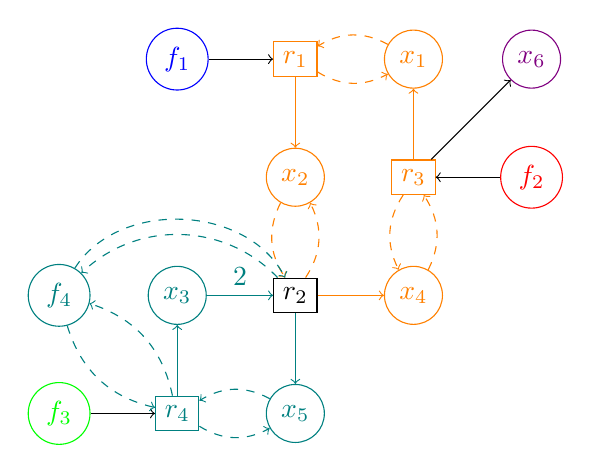
\begin{tikzpicture}
      \node[draw, circle, blue] (f1) at (-1.5,0) {$f_1$};      
      \node[draw, circle, red] (f2) at (3,-1.5) {$f_2$};
      \node[draw, circle, green] (f3) at (-3,-4.5) {$f_3$};
      \node[draw, teal, circle] (f4) at (-3,-3) {$f_4$};
            
      \node[draw, orange, circle] (x1) at (1.5,0) {$x_1$};			
      \node[draw, orange, circle] (x2) at (0,-1.5) {$x_2$};      
      \node[draw, teal, circle] (x3) at (-1.5,-3) {$x_3$};
      \node[draw, orange, circle] (x4) at (1.5,-3) {$x_4$};
      \node[draw, teal, circle] (x5) at (0,-4.5) {$x_5$};
      \node[draw, circle, violet] (x6) at (3,0) {$x_6$};
      
      \node[draw, orange, rectangle] (r1) at (0,0) {$r_1$};
      \node[draw, rectangle] (r2) at (0,-3) {$r_2$};
      \node[draw, orange, rectangle] (r3) at (1.5,-1.5) {$r_3$};
       \node[draw, teal, rectangle] (r4) at (-1.5,-4.5) {$r_4$};
      
      \draw[->] (f1) to (r1);
      \draw[->, orange, dashed] (x1) to [bend right = 30] (r1);
      \draw[->, orange, dashed] (r1) to [bend right = 30] (x1);
      \draw[->, orange]  (r1) to (x2);
      \draw[->, orange, dashed] (x2) to [bend right = 30] (r2);	
      \draw[->, orange, dashed] (r2) to [bend right = 30] (x2);
      \draw[->, teal] (x3) to node[midway, above] {$2$} (r2);
      \draw[->, orange] (r2) to (x4);
      \draw[->, teal ] (r2) to (x5);
      \draw[->, orange, dashed] (x4) to [bend right = 30] (r3);
      \draw[->, orange, dashed] (r3) to [bend right = 30] (x4);
      \draw[->] (f2) to (r3);
      \draw[->, orange] (r3) to (x1);
      \draw[->] (r3) to (x6);
      \draw[->, teal, dashed] (x5) to [bend right = 30] (r4);
      \draw[->, teal, dashed] (r4) to [bend right = 30] (x5);      
      \draw[->] (f3) to (r4);
      \draw[->, teal, dashed] (f4) to [bend right = 30] (r4);
      \draw[->, teal, dashed] (r4) to [bend right = 30] (f4);
      
      \draw[->, teal, dashed] (f4) to [bend left = 60] (r2);
      \draw[->, teal, dashed] (r2) to [bend right = 45] (f4);      
      \draw[->, teal] (r4) to (x3);      
    \end{tikzpicture}
  \end{minipage}
  \caption{\textit{(Left):} Example of an irreducible, monocatalyzed RAF
    written as CRN reactions with a cut-vertex that has a single
    catalyst. Catalyzations are indicated in brackets. \textit{(Right):}
    Depiction of the corresponding König graph with catalyzations indicated
    as dashed lines. Different strong blocks are depicted in different
    colours, while the cut-vertices $r_2$, belonging to two strong blocks
    (teal and orange) is coloured black. For the teal strong block, $r_4$
    is the `$r^*$' reaction expected via Lemma \ref{lem:StrongBlocks} and
    for the orange strong block it is $r_2$.}
  \label{ex:CutVertex2}
\end{figure}

We refer to a reaction $r^*$ as in the statement of
Lemma~\ref{lem:StrongBlocks} as an \emph{entry reaction} for $\block$. By
an inspection of the example in Fig.~\ref{ex:CutVertex2} we \PFS{observe}
that such entry reactions appear in intimate relation with cut-vertices of
the bipartite graph $K(\mathcal{R}')$. For brevity, we investigate this
intuition only via the following two corollaries of
Lemma~\ref{lem:StrongBlocks}.  \vspace{6pt}
\begin{corollary}\label{cor:strongblock1}
  Let $\RAF$ be an irreducible monocatalyzed RAF. Let $\block$ be a maximal
  strong block of $K(\RAF)$ containing at least one species-vertex outside
  the food and waste sets, i.e.,
  $ X(\block)\not\subseteq \food\cup\mathbf{W}_{\RAF}.$ Further assume that
  there exists a species $\tilde{x}\notin\food\cup\mathbf{W}_{\RAF}$ with
  $\tilde{x}\notin\block$. Then every entry reaction $r^*$ of $\block$ has
  at least two distinct F-products..
\end{corollary}
\begin{proof}
  Consider any entry reaction $r^*$ of
  $\block$. Lemma~\ref{lem:StrongBlocks} yields that $r^*$ has an F-product
  $x_{\pi_1}$ in $\block$. In turn, via Lemma~\ref{lem:PSC}, there exists a
  directed path $\mathcal{P}$ in $K(\RAF)$ from $r^*$ to
  $\tilde{x}\not\in X(\block)$, with $\mathcal{P}\cap
  \food=\emptyset$. Since $\block$ is a strong block and
  $r^*\in \mathcal{R}(\block)$, it follows that
  $\mathcal{P}\cap \block=\{r^*\}$. Let $\tilde{\tilde{x}}$ be the first
  species-vertex after $r^*$ in $\mathcal{P}$. By construction,
  $\tilde{\tilde{x}}\not \in \mathbf{W}_{\RAF}$. Moreover, via Lemma
  \ref{lem:cutvert}, $\tilde{\tilde{x}}$ cannot be a cut-vertex and thus
  there exists a maximal strong block $\tilde{\block} \neq \block $ which
  contains both vertices $r^*$ and $\tilde{\tilde{x}}$.  If
  $\{r^*, \tilde{\tilde{x}}\}$ are the only two vertices in
  $\tilde{\block}$, then $\tilde{\tilde{x}}$ is an F-product of $r^*$, and
  we are done. Otherwise, there exists at least another reaction
  $\tilde{r}\in \mathcal{R}(\block)$, $\tilde{r}\neq r^*$. Indirectly
  assume there exists no F-product $x_{\pi_2}$ of $r^*$, which is not in
  $\block$. Arguing exactly as in the proof of Lemma
  \ref{lem:StrongBlocks}, starting from
  $\tilde{\mathbf{R}}_0=\{\tilde{\fr}\}$ and building a RAF via
  \eqref{RAFbuild}, we construct a nonempty
  $\RAF'\subseteq \RAF\setminus \fr^* \subset \RAF$, leading to
  contradiction.
\end{proof}
Corollary~\ref{cor:strongblock1} directly yields the following statement,
which gives an easy-to-check structural necessary condition for the
presence of multiple strong blocks involving species that are not in the
food or in the waste sets.  \vspace{6pt}
\begin{corollary}\label{cor:strongblock2}
  Let $\RAF$ be an irreducible monocatalyzed RAF. If every F-reaction
  $\fr\in\RAF$ satisfies
  \begin{equation}\label{eq:condmanysb}
    |\fproducts(\fr)|<2,
  \end{equation}
  then $K(\RAF)$ has a unique maximal strong block containing at least one
  species-vertex outside the food and waste sets.
\end{corollary}
\begin{proof}
  Immediate from Cor.~\ref{cor:strongblock1}.
\end{proof}
For example, if all F-reactions $\fr\in\RAF$ are of the form
\begin{equation*} 
  x_\rho + (x_\kappa)\quad\underset{\fr}{\longrightarrow}\quad
  x_\pi + (x_\kappa)
\end{equation*}
then \eqref{eq:condmanysb} is satisfied and thus $K(\RAF)$ is essentially
one single strong block. Here, `essentially' simply means by not
considering strong blocks involving only food and waste species.

\begin{figure}[htb]
	\begin{minipage}[c]{0.5\textwidth}
		\centering
	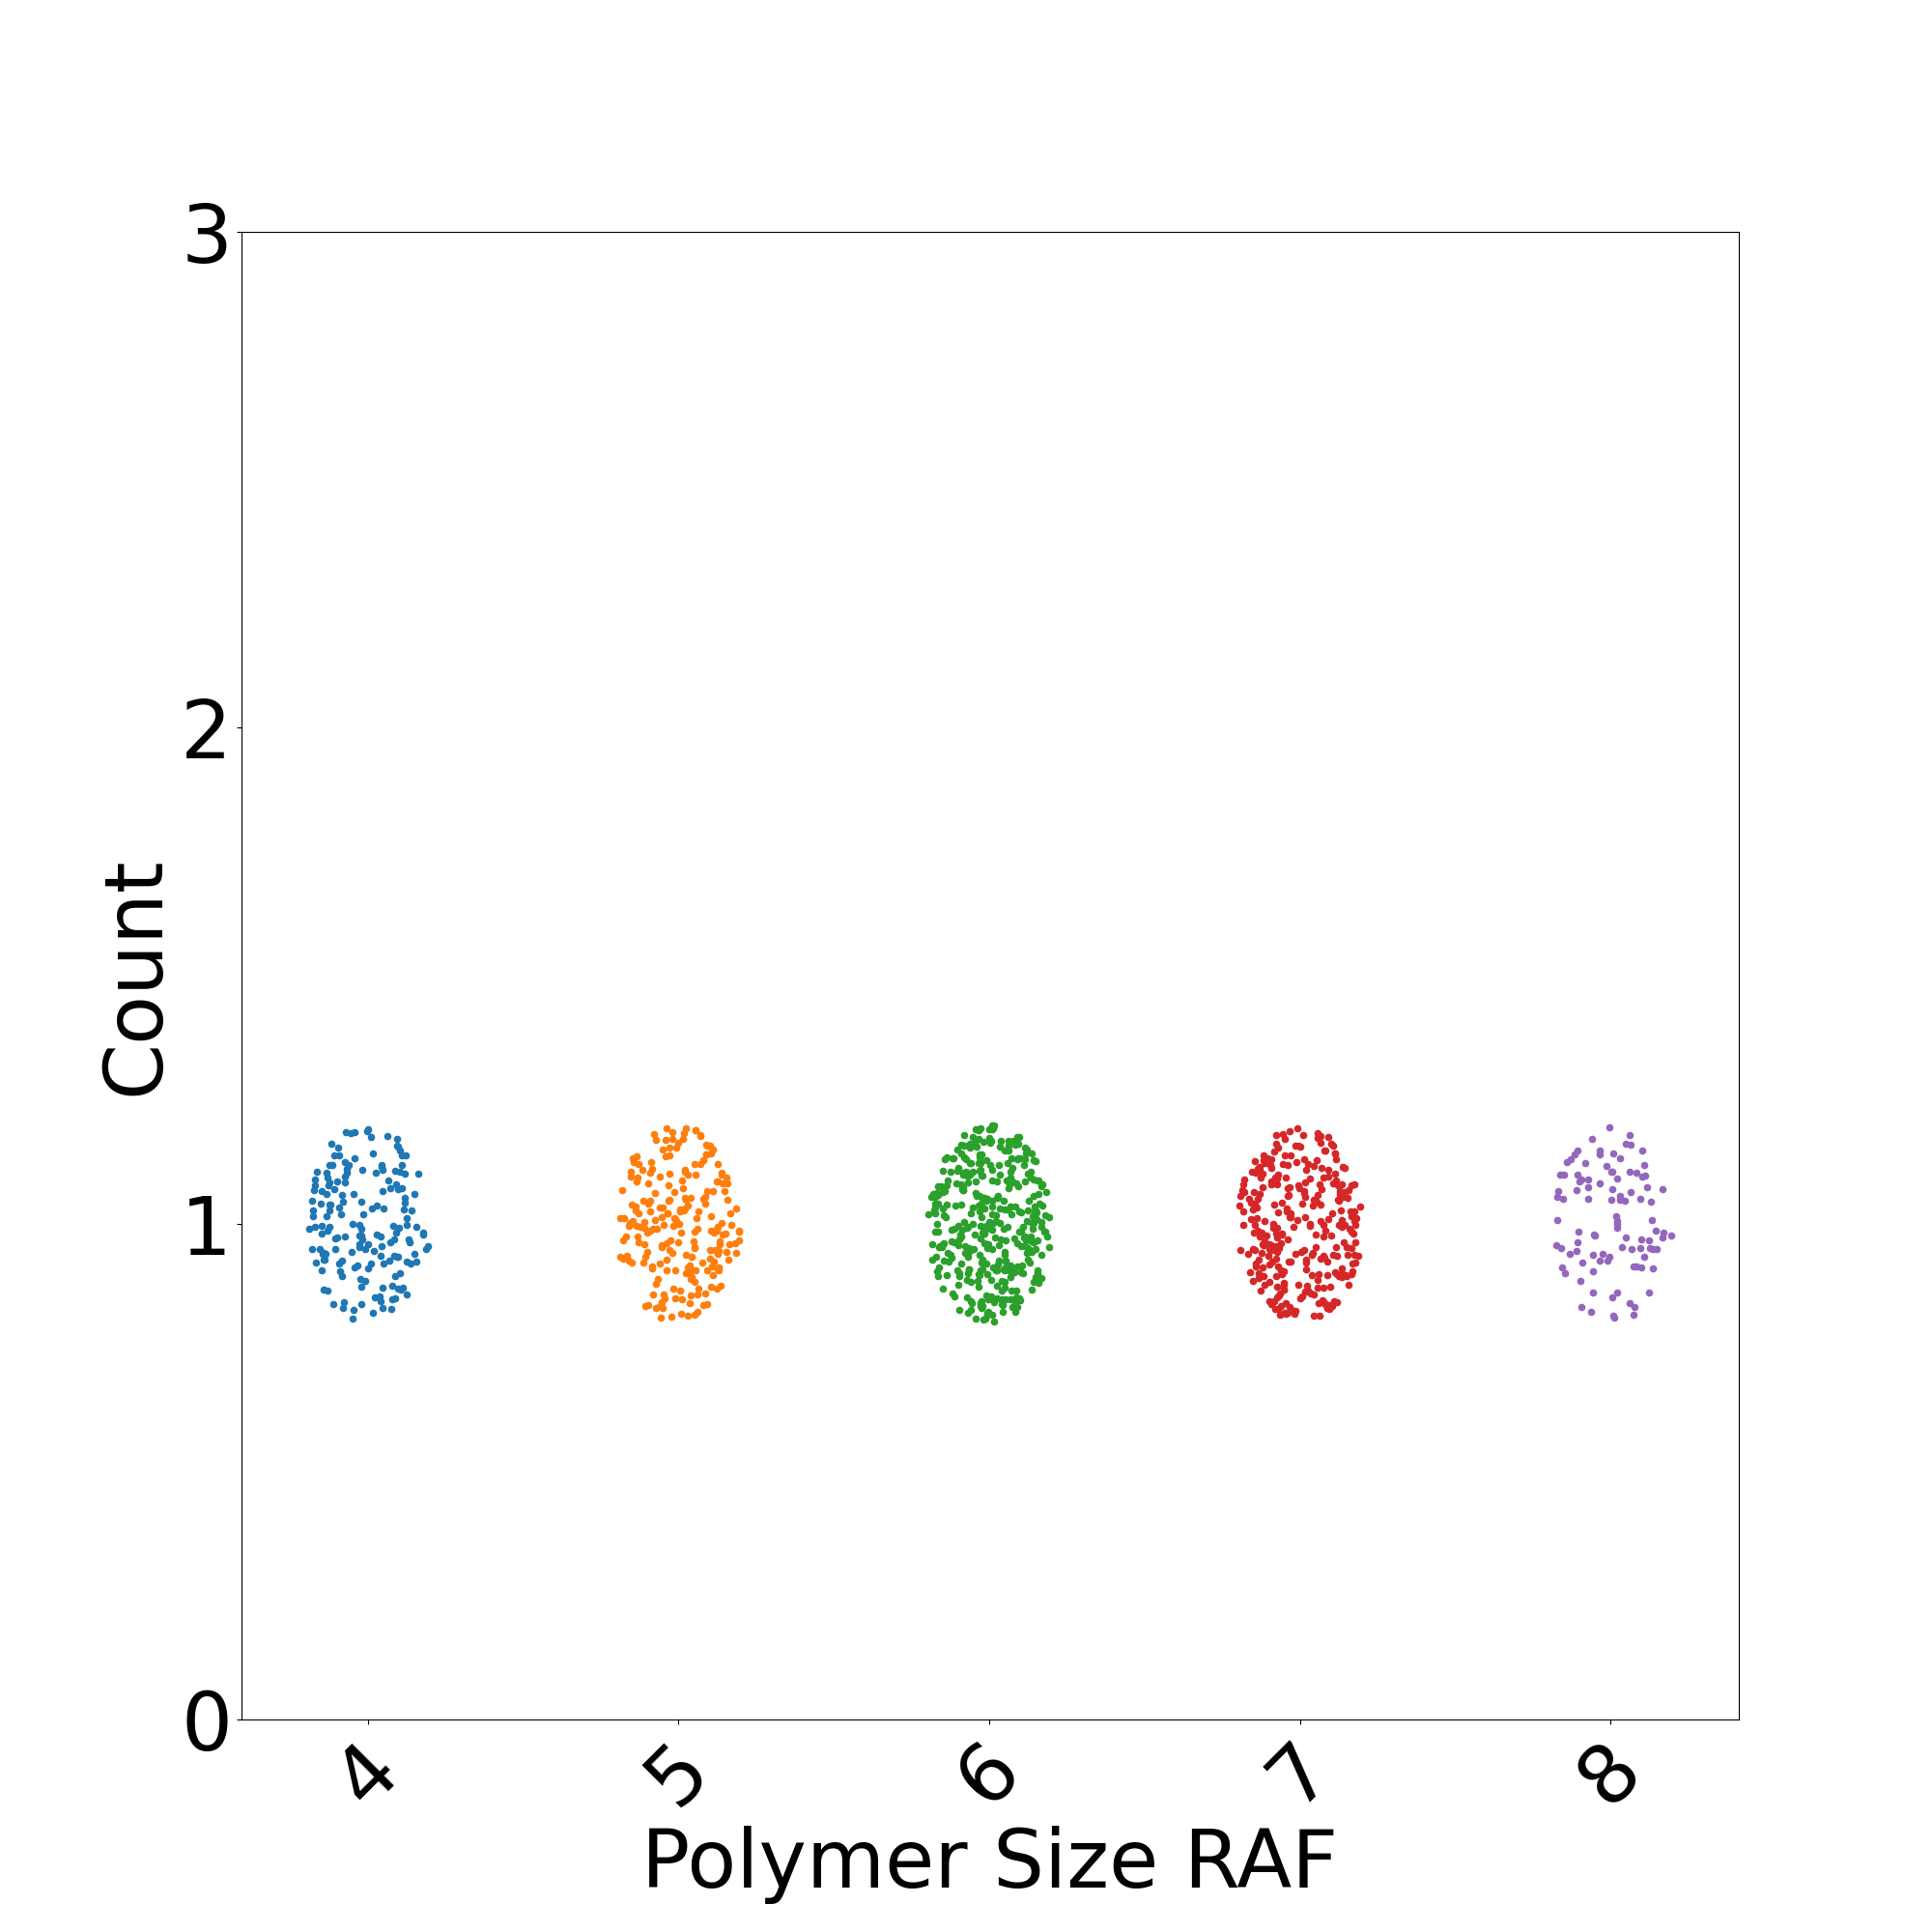
\includegraphics[width=\textwidth]{./Pictures/iRAFrevStrongBlocks.png}
	\end{minipage}%
	\hfill%
	\begin{minipage}[c]{0.5\textwidth}
		\centering
		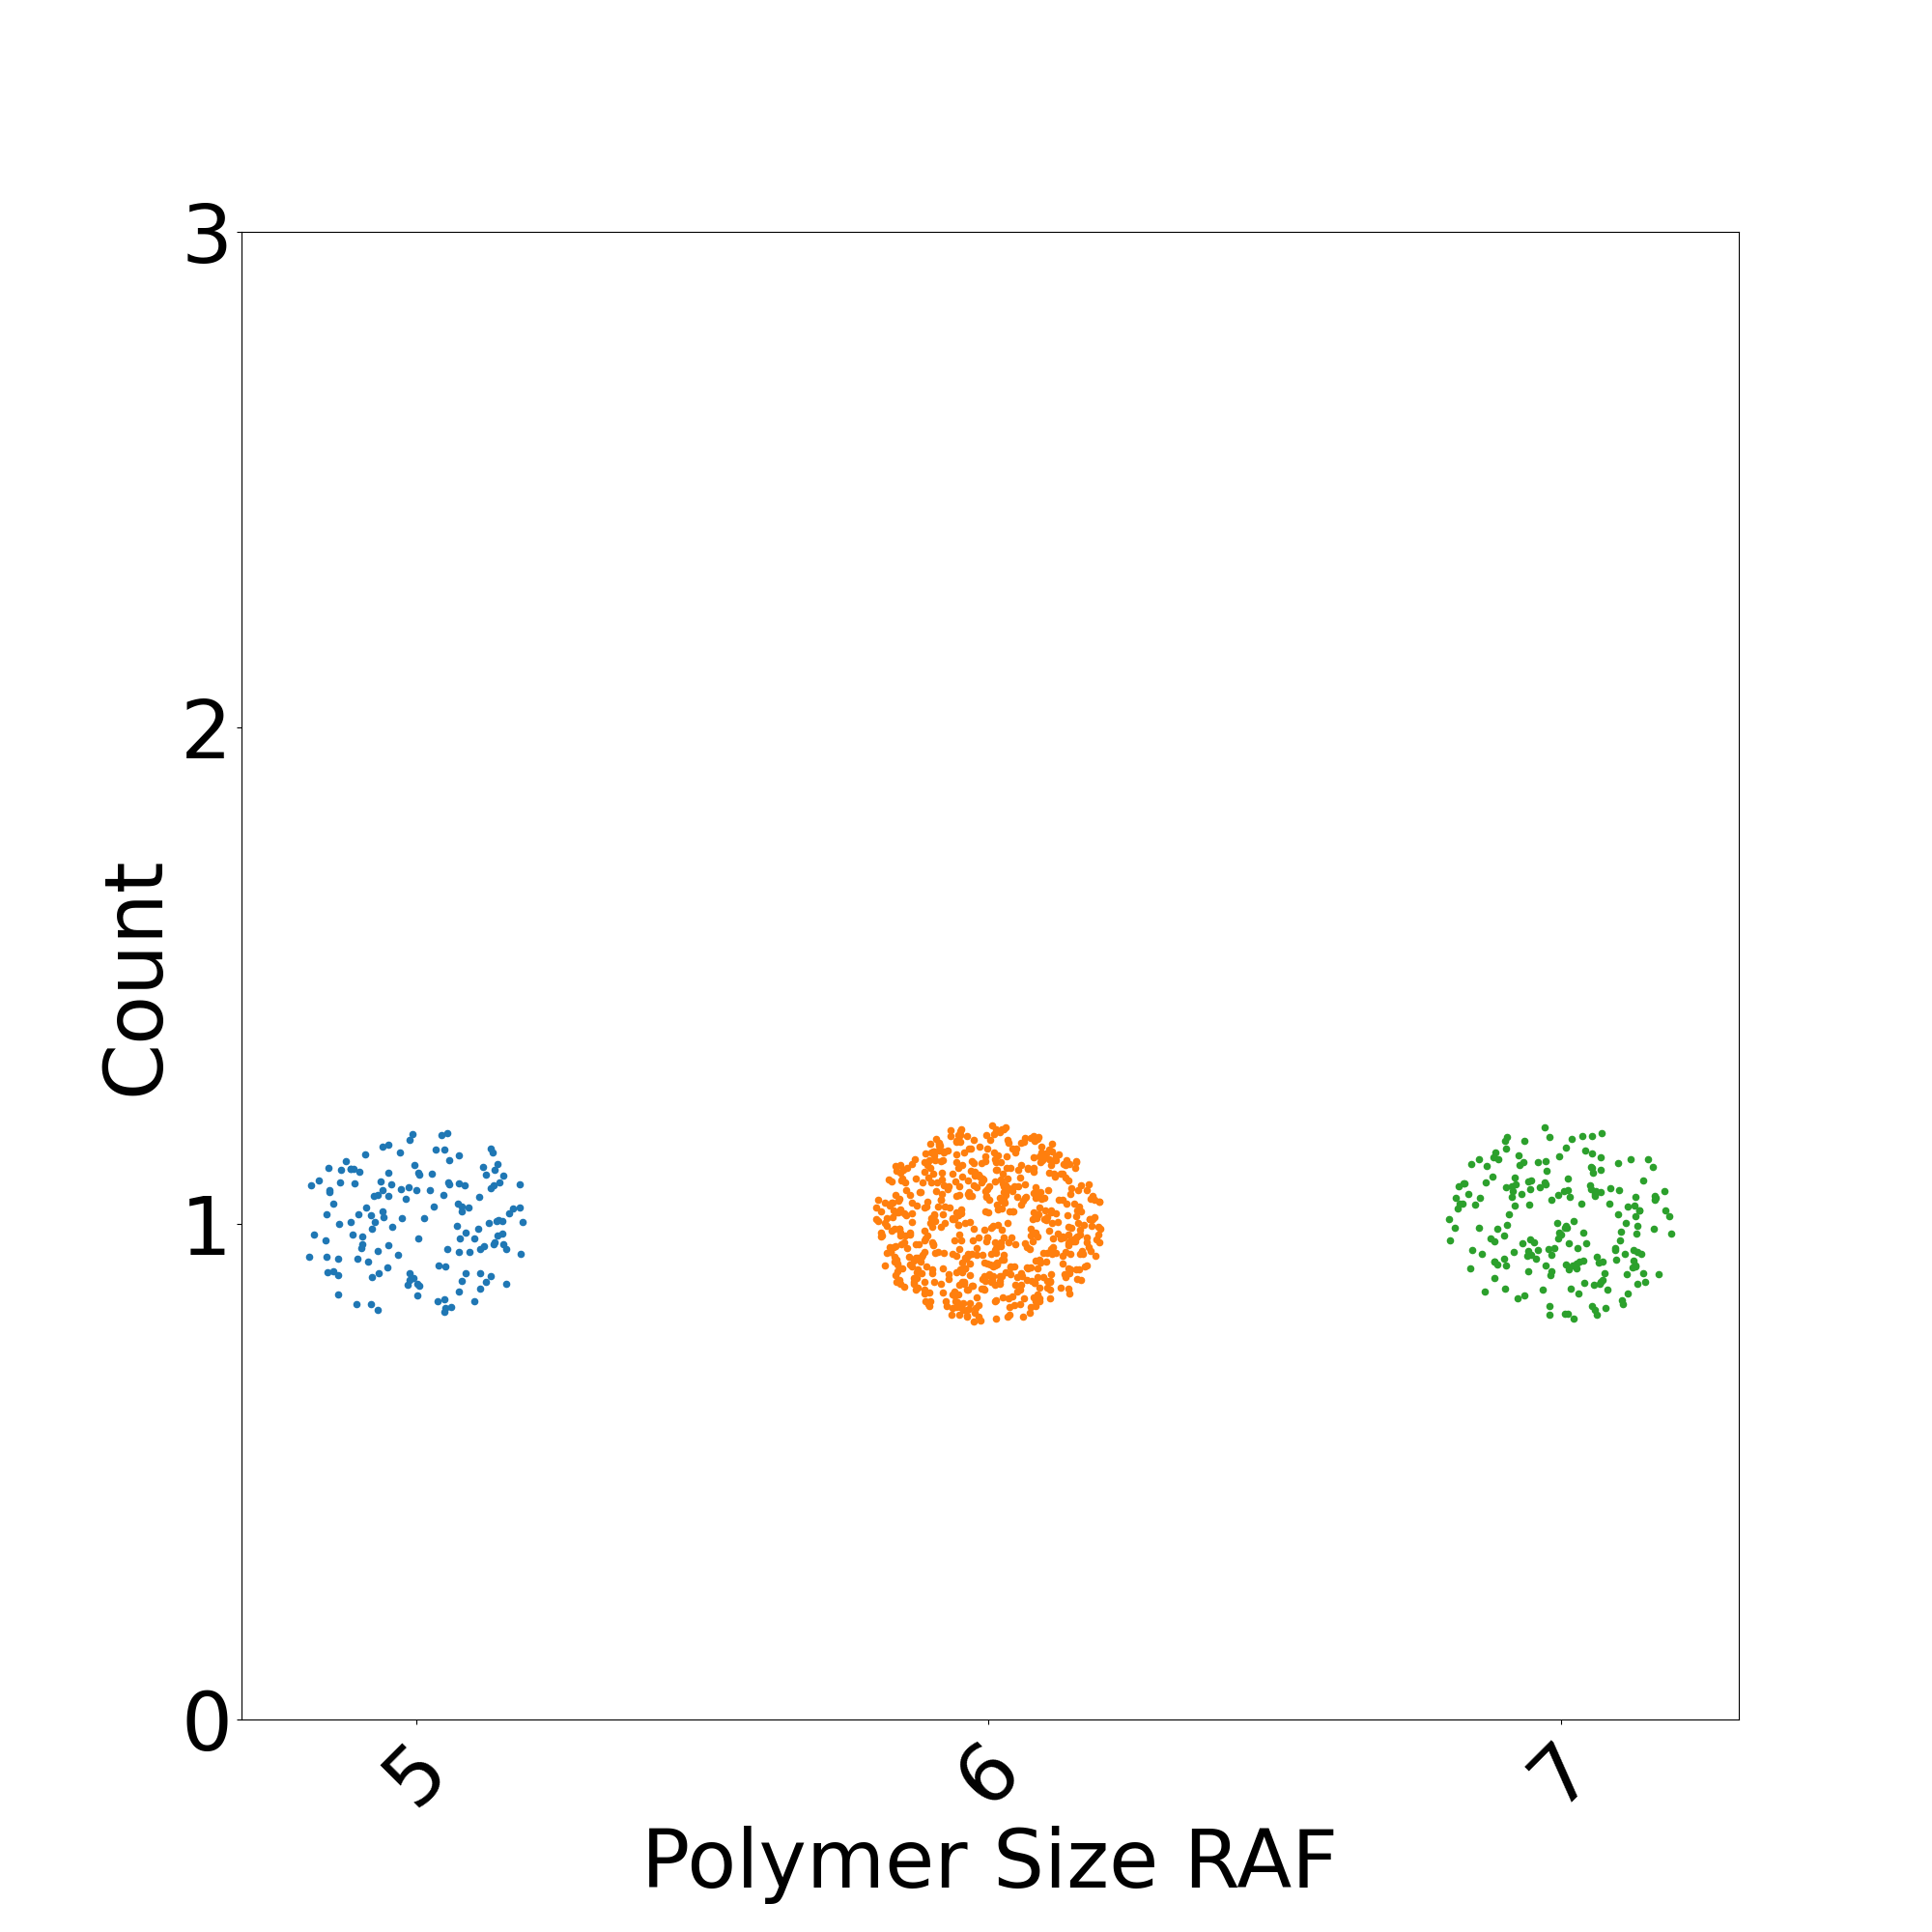
\includegraphics[width=\textwidth]{./Pictures/iRAFirrevStrongBlocks.png}
	\end{minipage}
	\caption{Number of strong blocks ....}
	\label{fig:StrongBlocks}
\end{figure}

\holy{Although RAFs can, in principle, be composed of multiple 
maximal strong blocks that contain at least one non-food, non-waste 
species-vertex, any irreducible RAF of the two instances of the binary 
polymer model depicted in Fig.~\ref{fig:irrRAFCores} consists of only 
one such block. According to Cor.~\ref{cor:strongblock2}, this is not 
surprising for instances containing only ligation F-reactions 
(Fig.~\ref{Fig:IrrRAFCores}, right panels), which all have only 
one F-product. However, even for the presence of both cleavage and 
ligation reactions, we could not find an instance for maximal polymer 
sizes of 5,6, and 7, where any of the collected irreducible RAF was 
composed of more than one maximal strong block that contained at 
least one non-food, non-waste species-vertex (see Fig.~\ref{S-fig:}\TODO{TBA}), 
although this is in principle possible as depicted in Fig.~\ref{fig:BPM}. 
The uniformly distributed probability of catalysis assignment results in 
densely connected networks, which was already reported in 
\TODO{Ask Wim for reference}. Nevertheless, the large number of 
autocatalytic cores in each irreducible RAF remains unexplained.}

Finally, we stress that entry reactions always identify a column in the
associated stoichiometric matrix
$S[X(\block)\setminus \food, \mathcal{R}(\block)]$ of
$\Gamma'=(\closure{\RAF}{\food},\mathcal{R}')$, restricted to the non-food
species in $\block$, which is nonnegative (property (i) in
Lemma~\ref{lem:StrongBlocks}) and it has at least one positive entry
(property (ii) in Lemma~\ref{lem:StrongBlocks}). Such an observation will
be pivotal to prove stoichiometric autocatalysis in each of such strong
blocks $\block$, as per our main result below. We proceed first by
introducing formally stoichiometric autocatalysis.

\section{Stoichiometric Autocatalysis}\label{sec:AutoCatIrrRAF}

In chemical reaction networks (CRN), a matrix-based definition of
\emph{stoichiometric autocatalysis} was introduced by Blokhuis et
al. \cite{blokhuis_Universal_2020} for networks without catalysis, and was
recently extended to the catalytic setting considered in the present paper
\cite{golnik_autocatalytic_2026}, where a reactant may also be a product of
the same reaction. The definition is as follows.

\vspace{6pt}
\begin{definition}\label{def:autSubRN}
  A CRN $\Gamma\coloneqq (X,\CR)$ is \emph{stoichiometric autocatalytic} if
  it contains a sub-CRN $\Gamma'=(X',\CR')$ such that
  \begin{enumerate}
  \item[i.] \emph{Well-formedness:} For any $r\in \mathcal{R}'$, there
    exists $x_1, x_2 \in X'$, not necessarily distinct, such that
    $s^-_{x_1r}s^+_{x_2r}\neq 0$;
  \item[ii.] \emph{Semi-positivity:} For the associated stoichiometric
    matrix $\SM'\coloneqq \SM[X',\CR']$ there exists
    $v\in \mathbb{R}_{>0}^{|\CR'|}$ such that $\SM'v>0$.
  \end{enumerate}
\end{definition}
\vspace{6pt}

A minimality concept for stoichiometrically autocatalytic CRN is expressed
in terms of subnetworks. A sub-CRN $\Gamma'$ that satisfies \textit{(i.)}
and \textit{(ii.)}, while no proper sub-CRN
$\Gamma''\subset\Gamma'$ %with X''\subset X', \CR''\subset \CR'$
does, is called an \emph{autocatalytic core}.  Any autocatalytic sub-CRN
thereby contains an autocatalytic core. The stoichiometric submatrix
associated to an autocatalytic core admits a reordering of the columns such
that all diagonal entries are nonpositive while all off-diagonal entries
are nonnegative \cite{blokhuis_Universal_2020, golnik_autocatalytic_2026, 
vassena_unstable_2024}. Matrices with
nonnegative off-diagonal entries are called \emph{Metzler matrices} in the
literature. An autocatalytic core of size $1$, i.e.,
$|X'|=|R'|=1$, is thus simply an \emph{autocatalytic reaction}
$r$ of the type:
\begin{equation}
    s^-_{x_1r}x_1+\ldots \quad\underset{r}\longrightarrow \quad s^+_{x_1r}x_2+\ldots\quad\quad\quad\text{with $s^+_{x_1r}>s^-_{x_1r}$.}
\end{equation}
By this simple example, it appears evident the quantitative role of the
stoichiometric coefficients in the definition of stoichiometric
autocatalysis (via the semipositivity condition). In RAF, in turn, the
quantitative value of the stoichiometry is irrelevant. However,
semipositivity of the stoichiometric matrix restricted to the non-food
molecules follows naturally for any food-generated set of reactions, as the
next lemma shows. \TODO{ADD SPECIFICATION ON THE F-REACTION ANNOYANCE}

\vspace{6pt}
\begin{lemma}~\label{lem:NonFoodSemipositiv2}
  Let $\mathcal{R}'$ be a food-generated set of reactions. Let $
  n:=\max\{\gamma(r)\mid r\in\CR'\}$, and for $k=1,\ldots,n$, define
  \begin{equation*}
    \mathcal{R}^k
    \coloneqq
    \{r\in\mathcal{R}'\mid \gamma(r)=k\},
    \qquad
    X^k
    \coloneqq
    \{x\in \closure{\mathcal{R'}}{\food}\setminus\food\mid \sgen(x)=k\}.
  \end{equation*}
  Pick any
  $\lambda=(\lambda_n,\ldots,\lambda_1)$ iteratively by choosing
  $\lambda_n>0$ and, for $k=n-1,\ldots,1$,
  \begin{equation*}
    \lambda_k
    > \max \left\{
      \max_{x\in X^k}
      \left[
        -\frac{
          \displaystyle
          \sum_{\ell=k+1}^{n}
          \lambda_\ell
          \sum_{r\in\mathcal{R}^\ell}\SM_{xr}
        }{
          \displaystyle
          \sum_{r\in\mathcal{R}^k}\SM_{xr}
        }
      \right],0 \right\},
  \end{equation*}
  and define $v\in \mathbb{R}^{|\mathcal{R}'|}_{>0}$ by $
  v_r\coloneqq \lambda_{\gamma(r)}.$
  Then
  \begin{equation*}
    \SM[\closure{\mathcal{R'}}{\food}\setminus\food,\mathcal{R}']v>0.
  \end{equation*}
  In particular,
  $\SM[\closure{\mathcal{R'}}{\food}\setminus\food,\mathcal{R}']$ is
  semi-positive.
\end{lemma}

\begin{proof}
  Arbitrarily take \(x\in \closure{\mathcal{R}'}{\food} \setminus\food\),
  and let \(k=\sgen(x)\). By the definition of species generation,
  $ \SM_{xr}=0$ for every $r\in\mathcal R^\ell,$ with $\ell<k,$ while
  $ \sum_{r\in\mathcal R^k}\SM_{xr}>0.$ Since \(v_r=\lambda_{\gamma(r)}\),
  it follows that
  \begin{equation*}
    \bigl(\SM[X'\setminus\food,\mathcal R']v\bigr)_x
    =
    \sum_{r\in\mathcal R'}\SM_{xr}v_r=
    \sum_{\ell=k}^{n}
    \lambda_\ell
    \sum_{r\in\mathcal R^\ell}\SM_{xr}
    =
    \lambda_k
    \sum_{r\in\mathcal R^k}\SM_{xr}
    +
    \sum_{\ell=k+1}^{n}
    \lambda_\ell
    \sum_{r\in\mathcal R^\ell}\SM_{xr}.
  \end{equation*}
  The defining condition on \(\lambda_k\) in the assumption of the Lemma
  directly yields
  \begin{equation*}
    \bigl(\SM[X'\setminus\food,\mathcal R']v\bigr)_x>0.
  \end{equation*}
  Since \(x\in X'\setminus\food\) is arbitrary,
  $\SM[X'\setminus\food,\mathcal R']v>0$. Since $v>0$ by construction,
  \(\SM[X'\setminus\food,\mathcal R']\) is semi-positive.
\end{proof}

Lemma~\ref{lem:NonFoodSemipositiv2} shows that semipositivity is a natural
property also for RAFs. Moreover, the structural result
Lemma~\ref{lem:StrongBlocks} yields the following theorem: each sub-CRN
$(X(\block)\setminus \food, \CR(\block))$, corresponding to a maximal,
non-trivial strong block $\block$ of $\king(\RAF)$ of an irreducible,
monocatalyzed RAF $\RAF$, is \emph{stoichiometrically autocatalytic}.

\vspace{6pt}
\begin{theorem}\label{Thm:StrBlockCore}
  Let $\RAF$ be an irreducible, monocatalyzed RAF, and let $\block$ be a
  maximal strong block $\king(\RAF)$, which contains a species-vertex $x^*$
  that is not not in the food and waste sets. Then $\block$ contains an
  autocatalytic core.
\end{theorem}
\vspace{6pt}

\begin{proof}
  We show that the subnetwork identified by $\block$ is stoichiometrically
  autocatalytic.
  \\
  Well-formedness follows naturally from the fact that any reaction-vertex
  $r$ in a strong-block $\block$ has at least one ingoing edge $(x_1,r)$
  and one outgoing edge $(r,x_2)$, with $x_1$ not necessarily distinct from
  $x_2$ but both $x_1,x_2\not\in \food \cup\mathbf{W}_{\RAF}$ via Lemma
  \ref{lem:StrongBlocks}.
  \\
  To show semi-positivity, consider an enlarged food
  set \begin{equation}\tilde{\food}:=\food\cup\{x\in
    \closure{\RAF}{\food}\;|\; x\not\in X(\block)\}.
  \end{equation}
  Lemma \ref{lem:StrongBlocks} guarantees that the set
  $\mathcal{R}(\block)$ is $\tilde{\food}$-generated as any entry reaction
  (with respect to the food set $\tilde{\food}$) $r^*$ has F-reactants only
  in $\tilde{\food}$. Since
  $\closure{\mathbf{R}'(\block}{\tilde{\food}})=X(\block)\setminus
  \tilde{\food}$, Lemma~\ref{lem:NonFoodSemipositiv2} yields semipositivity
  of $S[X(\block)\setminus \tilde{\food},\mathcal{R}(\block)]$ .
\end{proof}

\section{Two different kinds of examples.}
\label{sec:examples}

Thm.~\ref{Thm:StrBlockCore} guarantees that each maximal strong block that 
contains at least one species-vertex that does not represent a food or waste 
molecule is a stoichiometric autocatalytic sub-CRN. In addition, at least one 
autocatalytic core does not contain any food molecules. To this end, we constrained 
the CRNs generated from each irreducible RAF of random instances of the binary 
polymer model from FIg.~\ref{fig:fig:irrRAFCores} to include only non-food molecules. 
Importantly, as Fig.~\ref{FoodVsNonFood} shows, these restricted networks still
exhibit large numbers of autocatalytic cores, which is not attributable to large numbers 
of maximal strong blocks, as each such irreducible RAF comprises only one 
maximal strong block that contains at least one non-food, non-waste species-vertex. 

\begin{figure}
	\centering
	\begin{minipage}[c]{\textwidth}	
		\begin{minipage}[c]{0.5\textwidth}
			\centering
			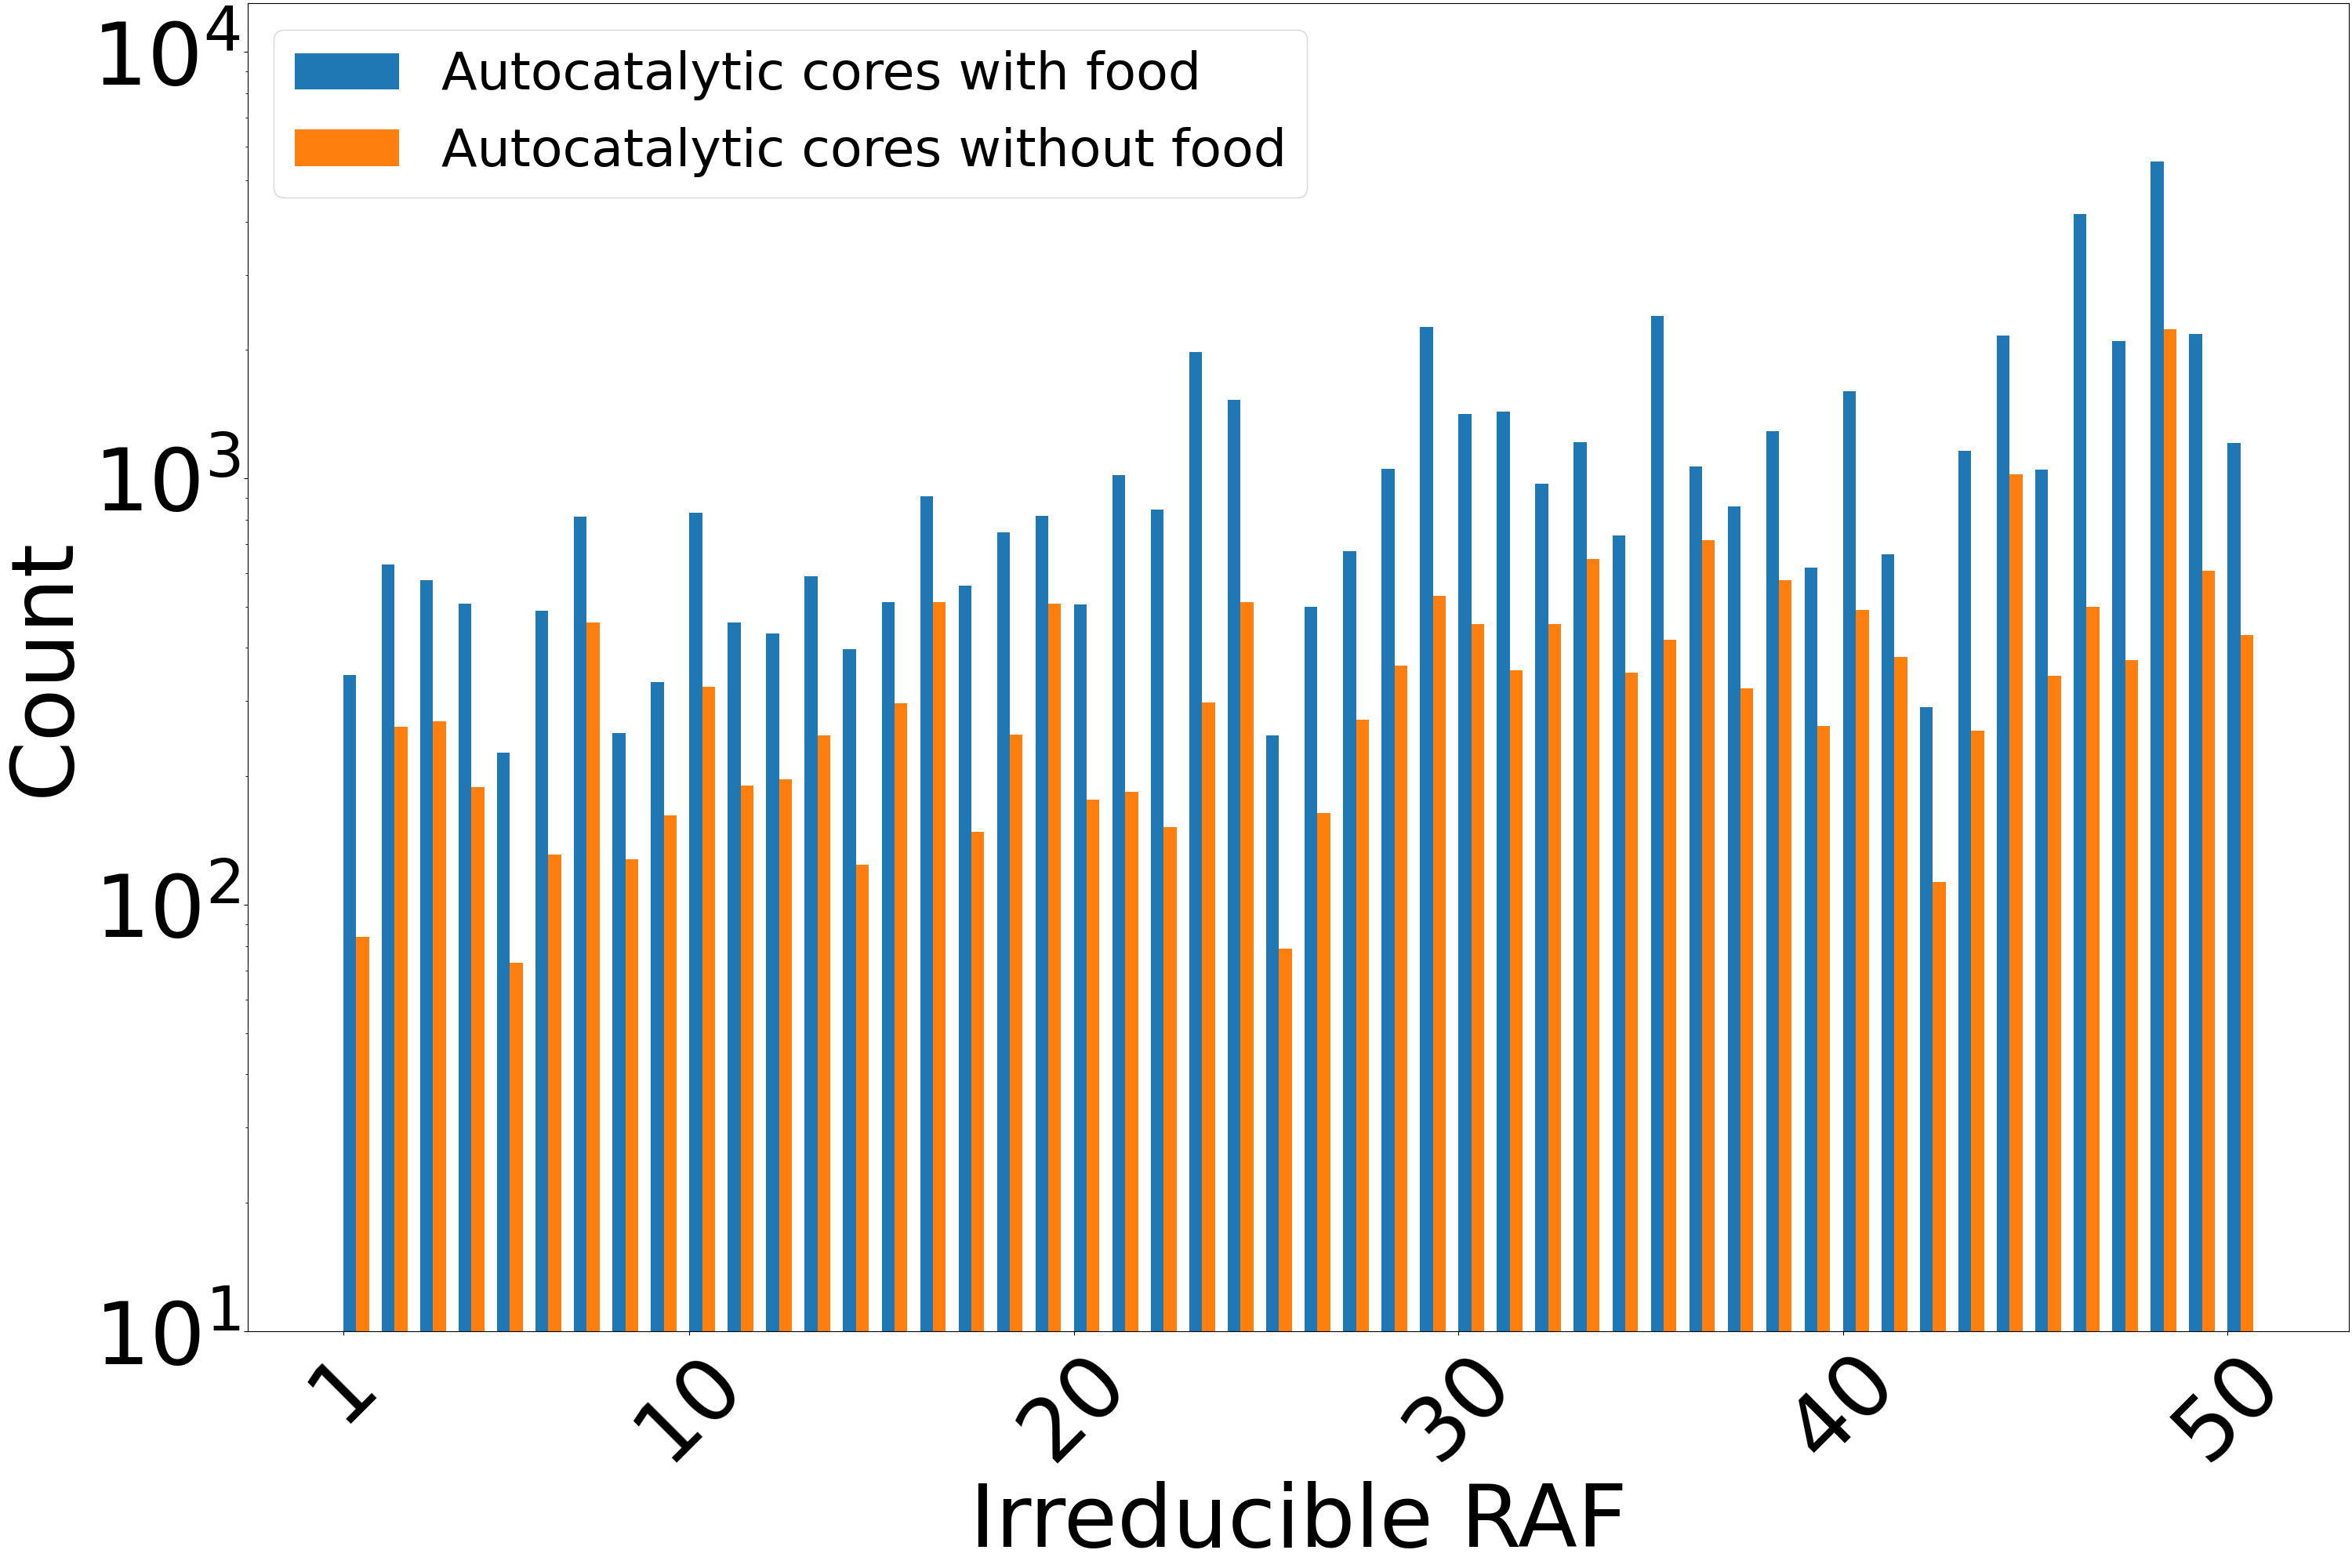
\includegraphics[width=\textwidth]{./Pictures/n6iRAFrevSplitWithVsWOFood.png}
		\end{minipage}%
		\hfill%
		\begin{minipage}[c]{0.5\textwidth}
			\centering
			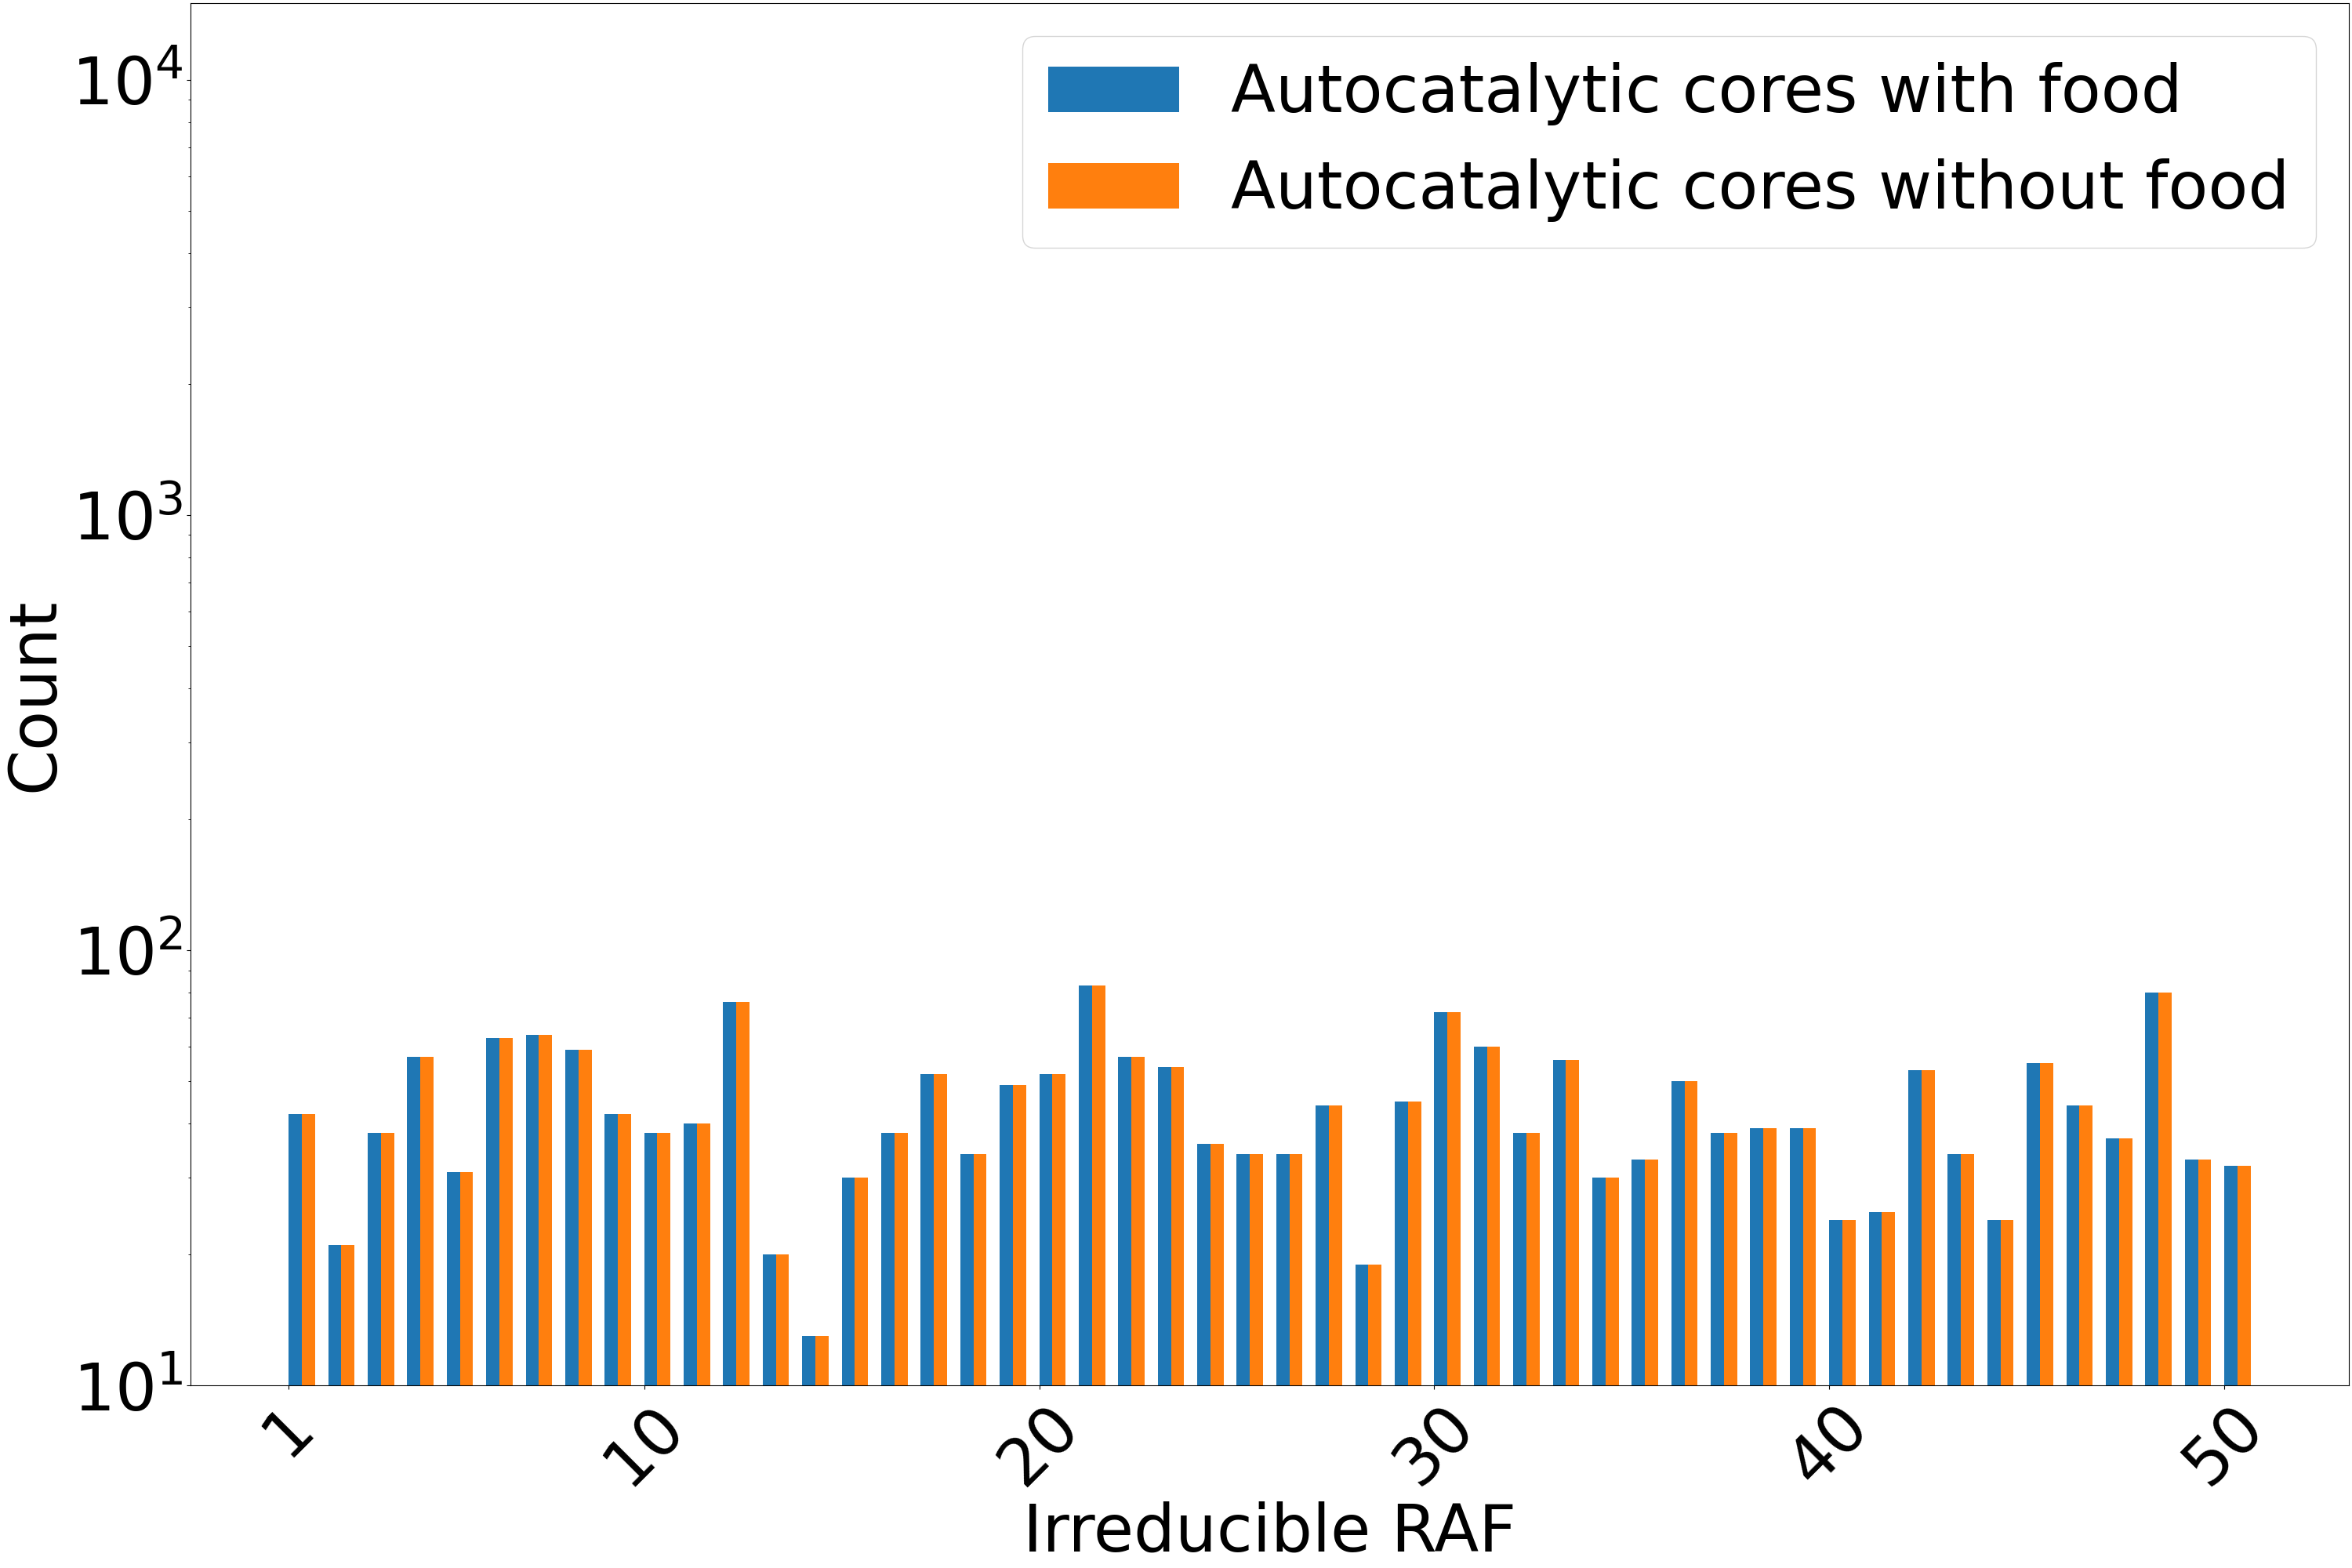
\includegraphics[width=\textwidth]{./Pictures/n6iRAFirrevCoresWvsWOFood.png}
		\end{minipage}
	\end{minipage}

	
	\caption{Autocatalytic cores in different irreducible RAFs from two independent instances 
	of the binary polymer model (see Fig.~\ref{fig:irrRAFCores} and Sect.~\ref{S-sec:BinPol}) with 
	and without food molecules.}
	\label{fig:FoodVsNonFood} 
\end{figure}

\TODO{***}

\begin{figure}
	\begin{minipage}[c]{\textwidth}
		\begin{minipage}[l]{0.5\textwidth}
			\begin{equation*}
				\begin{split}
					r_1&: f + (x_1) \rightarrow x_2 + (x_1)\\[0.5em]
					r'_2&: x_2 + (x'_2) \rightarrow x_3 + (x'_2) \\[0.5em]
					r''_2&: x_2 + (x''_2) \rightarrow x_3 + (x''_2) \\[0.5em]
					r'_3&: x_3 + (x'_3) \rightarrow x_4 + x'_2 + x''_2 + (x'_3) \\[0.5em]
					r''_3&: x_3 + (x''_3) \rightarrow x_4 + x'_2 + x''_2 + (x''_3) \\[0.5em]
					& \hspace{3pt} \vdots \\[0.5em]
					r_n&:  x_n + (x'_n) \rightarrow x_1 + x'_{n-1} + x''_{n-1} + x'_n + (x'_n) \\[0.5em]
				\end{split}
			\end{equation*}
		\end{minipage}%
		\hfill%
		\begin{minipage}[r]{0.5\textwidth}
			\begin{equation*}
				\SM=
					\begin{pmatrix} 
						0 		& 0  		& 	0 		& 	0 		& \ldots 	& 	0	& 1 \\ 
						1 		& -1 		& 	0 		& 	0 		& \ldots 	&	0	& 0 \\
						0 		& 0  		& 	1 		& 	0 		& \ldots 	& 	0	& 0 \\
						0 		& 0  		& 	1 		& 	0 		& \ldots 	& 	0	& 0 \\
						0 		& 1 	 	& 	-1 		& 	0 		& \ldots 	& 	0	& 0 \\
						0 		& 0		&	0		& 	1 		& \ldots 	& 	0	& 0 \\
						0 		& 0		&	0		&	 1 		& \ldots 	& 	0	& 0 \\
						0 		& 0		&	1		& 	-1 		& \ldots 	& 	0	& 0 \\
						\vdots	& \vdots	&	\vdots	&	\vdots 	& \ddots	& 	-1	& 0\\
						0		& 0		&	0		&	0 		& \ldots	& 	0	& 1\\
						0		& 0		&	0		&	0 		& \ldots	& 	0	& 1\\
						0		& 0		&	0		&	0 		& \ldots	& 	1	& -1\\
					\end{pmatrix}
			\end{equation*}
		\end{minipage}
	\end{minipage}
	\hfill
	\begin{minipage}[c]{\textwidth}
		\centering
		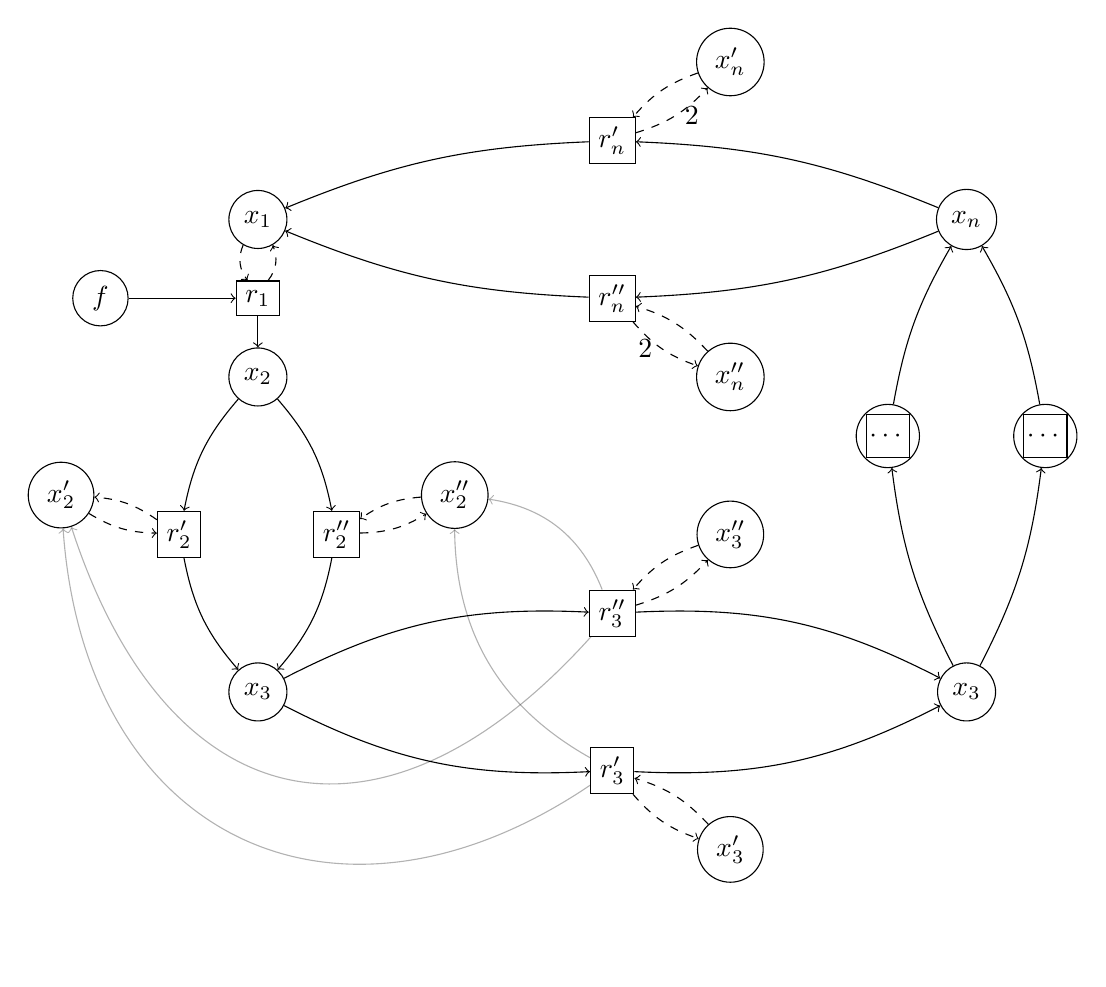
\begin{tikzpicture}
			\node[draw, circle] (f) at (-1,0) {$f$};
			\node[draw, circle] (x1) at (1,1) {$x_1$};
			\node[draw, circle] (x2) at (1,-1) {$x_2$};
			\node[draw, circle] (x'2) at (-1.5,-2.5) {$x'_2$};
			\node[draw, circle] (x''2) at (3.5,-2.5) {$x''_2$};
			\node[draw, circle] (x3) at (1,-5) {$x_3$};
			\node[draw, circle] (x'3) at (7,-7) {$x'_3$};
			\node[draw, circle] (x''3) at (7,-3) {$x''_3$};
			\node[draw, circle] (x4) at (10,-5) {$x_3$};
			\node[draw, circle] (xn) at (10,1) {$x_n$};			
			\node[draw, circle] (x'n) at (7,3) {$x'_n$};
			\node[draw, circle] (x''n) at (7,-1) {$x''_n$};
			
			\node[draw, rectangle] (r1) at (1,0) {$r_1$};
			\node[draw, rectangle] (r'2) at (0,-3) {$r'_2$};
			\node[draw, rectangle] (r''2) at (2,-3) {$r''_2$};			
			\node[draw, rectangle] (r'3) at (5.5,-6) {$r'_3$};
			\node[draw, rectangle] (r''3) at (5.5,-4) {$r''_3$};
			
			\node[draw, minimum size=0.55cm] (r'k) at (9,-1.75) {};
			\node[draw, minimum size=0.55cm] (r''k) at (11,-1.75) {};
			\node[draw, circle] (r'k) at (9,-1.75) {$\cdots$};
			\node[draw, circle] (r''k) at (11,-1.75) {$\cdots$};			
			
			\node[draw, rectangle] (r'n) at (5.5,2) {$r'_n$};
			\node[draw, rectangle] (r''n) at (5.5,0) {$r''_n$};			
			
			\draw[->] (f) to (r1);
			\draw[->, dashed] (x1) to [bend right = 30](r1);
			\draw[->, dashed] (r1) to [bend right = 30] (x1);
			\draw[->] (r1) to (x2);
			\draw[->] (x2) to [bend right = 15] (r'2);
			\draw[->] (x2) to [bend left = 15] (r''2);			
			\draw[->, dashed] (x'2) to [bend right = 15] (r'2);
			\draw[->, dashed] (r'2) to [bend right = 15] (x'2);
			\draw[->, dashed] (x''2) to [bend right = 15] (r''2);
			\draw[->, dashed] (r''2) to [bend right = 15] (x''2);			
			\draw[->] (r'2) to [bend right = 15] (x3);
			\draw[->] (r''2) to [bend left = 15] (x3);
			
			\draw[->] (x3) to [bend right=15] (r'3);
			\draw[->] (x3) to [bend left=15] (r''3);
			\draw[->] (r'3) to [bend right=15] (x4);
			\draw[->] (r''3) to [bend left=15] (x4);			
			\draw[->, opacity=0.3] (r''3) to [bend right = 30] (x''2);
			\draw[->, opacity=0.3] (r'3) to [bend left=60, looseness=1.35] (x'2);
			\draw[->, opacity=0.3] (r'3) to [bend left = 30] (x''2);
			\draw[->, opacity=0.3] (r''3) to [bend left=60, looseness=1.5] (x'2);
			
			\draw[->, dashed] (x'3) to [bend right=15] (r'3);
			\draw[->, dashed] (r'3) to [bend right=15] (x'3);
			\draw[->, dashed] (x''3) to [bend right=15] (r''3);
			\draw[->, dashed] (r''3) to [bend right=15] (x''3);
						
			\draw[->] (x4) to [bend left=10] (r'k);
			\draw[->] (x4) to [bend right=10] (r''k);
			
			\draw[->] (r'k) to [bend left=10] (xn);
			\draw[->] (r''k) to [bend right=10] (xn);
			
			\draw[->] (xn) to [bend right=10] (r'n);
			\draw[->] (xn) to [bend left=10] (r''n);
			
			\draw[->] (r'n) to [bend right=10] (x1);
			\draw[->] (r''n) to [bend left=10] (x1);
			
			\draw[->, dashed] (r'n) to [bend right=15] node[midway, right]{$2$} (x'n);
			\draw[->, dashed] (x'n) to [bend right=15] (r'n);
			
			\draw[->, dashed] (r''n) to [bend right=15] node[midway, left]{$2$} (x''n);
			\draw[->, dashed] (x''n) to [bend right=15] (r''n);
											
		\end{tikzpicture}		
	\end{minipage}
	\caption{The necklace RAF}
	\label{fig:NecklaceRAF}
\end{figure}


\section{Discussion}

\textsc{Reflexively autocatalytic sets (RAFs)} and \emph{stoichiometric
  autocatalysis} are grounded in different formalizations of chemical
reaction systems that lead to inequivalent concepts of reactions,
distinguished by the manner in which catalysis is handled. While in CRNs,
underlying the theory of \emph{stoichiometric autocatalysis}, catalysts are
not formally distinguished from other reactants and products, the CRS
framework focuses on net F-reactions, considering catalysts as external to
the F-reactions. In addition, in CRS, species can appear on both sides of
the stoichiometric equation without being considered a catalyst. As a
consequence, F-reactions are equivalence classes of (CRN) reactions with
respect to the equivalence relation $\sim$ (Eq.~\eqref{eq:EqRel}),
describing reactions that share the same non-catalyst reactants
(F-reactants) and the same non-catalyst products (F-products), with
identical stoichiometries, see Sec.~\ref{sec:CRNCRS}.

From a set of CRN reactions $\CR$, the set of corresponding F-reactions
$\FR$ can be obtained as the quotient set of $\CR$, i.e.
\begin{equation}
  \FR=\CR/\mathord{\sim}.
\end{equation} 
This implies that the CRS
$\mathbf{\Phi}(\Gamma)= (X, \CR/\mathord{\sim},
\kappa_F(\CR/\mathord{\sim}))$, with $\kappa_F(\CR/\mathord{\sim})$
determined as described in Eq.~\eqref{eq:CatCFR}, reflects the quotient
structure of the CRN $\Gamma=(X, \CR)$. In turn, the reactions of the CRN
$\Gamma(\mathbf{\Phi})$ associated with a given CRS
$\mathbf{\Phi}\coloneqq (X, \FR, \kappa_F(\FR))$ can be obtained from
$\kappa_F(\FR)$, since each catalyzation of an F-reaction specifies a
unique CRN reaction. In case each F-reaction is associated with a single
catalyzation (monocatalyzation), CRN and F-reactions are in one-to-one
correspondence; each equivalence class consists of a single element.

Although inherently distinct, it was recently demonstrated that every
\textsc{RAF} that is not a \textsc{CAF} is \emph{stoichiometrically
  autocatalytic} \cite{golnik_bridging_2026}. In the present contribution,
we examine this relationship in greater detail, focusing in particular on
the interplay between the minimal structures arising in both frameworks,
i.e., \textsc{irreducible RAFs} and \emph{autocatalytic
  cores}. \PFS{Analyzing irreducible RAFs}obtained from random instances of
the binary polymer model \cite{kauffman_autocatalytic_1986} \PFS{with}
\texttt{autogatito}, \PFS{we observed} an unexpectedly large \PFS{number}
of autocatalytic cores in each irreducible RAF
(Fig.~\ref{fig:irrRAFCores}). \PFS{This observation cound not be explained}
by the theoretical results stated in \cite{golnik_bridging_2026}.

\emph{Autocatalytic cores} correspond to \emph{fluffles} in the bipartite
K\H{o}nig graph -- that is, strongly connected blocks containing equal
numbers of species and reaction vertices, in which every species vertex has
out-degree~1, and every reaction vertex has in-degree~1 (F1--F3). It seemed
natural, therefore, to identify analogous patterns in irreducible RAFs. As
CRN and CRS can be canonically identified with each other whenever each
equivalence class is trivial, we focused on monocatalyzed, irreducible RAFs
$\RAF$. This allowed us to investigate their properties by examining the
structure of the bipartite K\H{o}nig graph $\king(\RAF)$ of the
corresponding CRN representation.

Irreducibility endows $\king(\RAF)$ with three fundamental properties for
any irreducible, monocatalyzed RAF $\RAF$
(Lemmata~\ref{lem:PSC}--\ref{lem:StrongBlocks}).
\begin{itemize}
\item[I1.] The subgraph of $\king(\RAF)$ induced by all species that are
    neither food nor waste is strongly connected.
\item[I2.] Every cut vertex of $\king(\RAF)$ is a reaction.
\item[I3.] Every strong block $\block$ of $\king(\RAF)$ that is
  non-trivial, i.e., not a single species vertex nor a digon composed of a
  reaction and a food species, contains a reaction $r^*$, also referred to
  as \emph{entry reaction}, that exertes the function of an inflow reaction
  for $\block$ -- that is, all F-reactants of $r^*$ are located outside, at
  least one F-product and one F-catalyst that is not a food-species is
  located inside, and $r^*$ has the lowest generation order among all
  reactions of $\block$.
\end{itemize}
Properties I1 and I2 imply a partition of $\king(\RAF)$ into strong blocks
that are separated by reaction vertices. Property I3 guarantees that each
of the non-trivial strong blocks is \emph{stoichiometrically
  autocatalytic}.

In fact, strong blocks are, by definition, well-formed. In addition,
\emph{entry reactions}, which have only F-catalysts as reactants and at
least one F-product inside the corresponding block $\block$, induce a
nonnegative column in the stoichiometric submatrix
$\SM[X(\block),\CR(\block)]$. This alone is indeed sufficient to guarantee
that $\SM[X(\block),\CR(\block)]$ for any non-trivial, strong block
$\block$ is semi-positive (Lemma~\ref{lem:NonFoodSemipositiv} and
Cor.~\ref{cor:blockSemiPositiv}). Well-formedness and semipositivity of the
associated stoichiometric submatrix -- the required conditions for a
sub-CRN to be autocatalytic (Def.~\ref{def:autSubRN}) -- yield that each
block is \emph{stoichiometrically autocatalytic} and therefore contains an
autocatalytic core (Thm.~\ref{Thm:StrBlockCore}).

\begin{figure}[bth]
  \begin{minipage}[c]{0.49\textwidth}
    \begin{equation}
      \begin{split}
	r_1& : f_1 + (x_1) \rightarrow  x_2 + (x_1) \\
	r_2& : f_2 + (x_4)\rightarrow x_3 + (x_4)\\
	r_3& : 2x_3 + (x_2) \rightarrow x_1 + x_4 + (x_2)
      \end{split}
    \end{equation}
  \end{minipage}%
  \hfill%
  \begin{minipage}[c]{0.49\textwidth}
    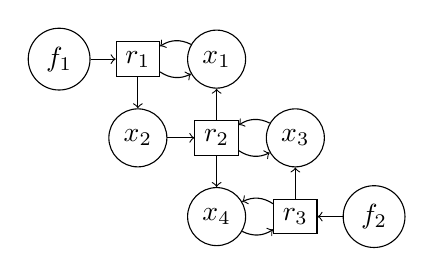
\begin{tikzpicture}
      \node[draw, circle] (f1) at (0,0) {$f_1$};
      \node[draw, circle] (f2) at (4,-2) {$f_2$};
      \node[draw, circle] (x1) at (2,0) {$x_1$};			
      \node[draw, circle] (x2) at (1,-1) {$x_2$};
      \node[draw, circle] (x3) at (3,-1) {$x_3$};
      \node[draw, circle] (x4) at (2,-2) {$x_4$};
      
      \node[draw, rectangle] (r1) at (1,0) {$r_1$};
      \node[draw, rectangle] (r2) at (2,-1) {$r_2$};
      \node[draw, rectangle] (r3) at (3,-2) {$r_3$};
      
      \draw[->] (f1) to (r1);
      \draw[->] (f2) to (r3);
      \draw[->] (x1) to [bend right = 30] (r1);
      \draw[->] (r1) to [bend right = 30] (x1);
      \draw[->] (r1) to (x2);			
      \draw[->] (x2) to (r2);
      \draw[->] (x3) to [bend right] (r2);
      \draw[->] (r2) to [bend right] (x3);
      \draw[->] (r2) to (x1);
      \draw[->] (r2) to (x4);
      \draw[->] (x4) to [bend right = 30] (r3);
      \draw[->] (r3) to [bend right = 30] (x4);
      \draw[->] (r3) to (x3);
    \end{tikzpicture}
  \end{minipage}
  \caption{\textit{(Left):} Example of an irreducible, monocatalyzed RAF
    written as CRN reactions with a cut-vertex that has a single
    catalyst. Catalyzations are indicated in brackets. \textit{(Right):}
    Depiction of the corresponding König graph.}
  \label{ex:CutVertex3}
\end{figure}

Independent of the structure of a core, different catalyzations can give
rise to equivalent autocatalytic cores. In fact, each autocatalytic core is
an element of equivalence classes that contain sub-CRNs on the same set of
species vertices and sets of reaction vertices that share the same set of
F-reactions (see Eq.~\eqref{eq:CoreEquiv}). The size of such an
$\simeq$-equivalence class grows exponentially with the product of the
sizes of $\sim$-equivalence classes of participating reactions
(Prop.~\ref{prop:ExpoNoCores}), which correlates with the large number of
autocatalytic cores observed and the reduced number of $\simeq$-equivalence
classes (Fig.~\ref{fig:UniqueFReactionCores}) in irreducible RAFs of random
instances of the binary polymer model \cite{kauffman_autocatalytic_1986}.

Even though all elements of the same $\simeq$-equivalence class are
autocatalytic whenever one element is autocatalytic, not all of them are
necessarily cores. The example illustrated in Fig.~\ref{fig:Minimality}
demonstrates how catalyzations impact the minimality property of
autocatalytic cores, as one element of an equivalence class is a core,
while the other is not. This observation originates from the way catalysts
are handled within CRNs, i.e., as reactants and products directly
participating in a reaction and thereby affecting the uniqueness of
reactants for each reaction inside a core.

\PFS{The results obtained here demonstrate that there are meaningful connections between the CRS and CRN formalisms that translate into strong similarities between two different notions of autocatalysis, in particular between \textsc{irreducible RAFs} and \emph{autocatalytic cores}. Although our results yield astonishing insights as well as useful implications, they are still far from establishing 1-to-1 correspondences between concepts in the two alternative formal frameworks. While the present results in essence characterize minimal RAFs in terms of CRNs, the converse, i.e., a characterization of autocatalytic cores in the language of CRS, remains an open research project.}

\bibliography{RAFCores}

\end{document}
